\documentclass[a4paper,leqno]{article}
\usepackage[utf8]{inputenc}
\usepackage{lmodern}
\usepackage{microtype}
\usepackage[inline]{enumitem}

\usepackage{siunitx}
\usepackage{multirow}
\usepackage{subcaption}

\usepackage[english]{babel}
\usepackage[autostyle, english=british]{csquotes}
\MakeOuterQuote{"}

\usepackage{commath}
\usepackage{amsmath}
\usepackage{amsthm}
\usepackage{amssymb}
\usepackage{mathtools}

\usepackage[dvipsnames]{xcolor}
\usepackage{pgfplots}
\pgfplotsset{compat=1.11}
\usepgfplotslibrary{fillbetween}
\usetikzlibrary{patterns}
\usetikzlibrary{arrows}

\newcommand*{\SectorRadius}{1.5ex}
\newcommand*{\SectorHalfAngle}{45}
\newcommand*{\SectorLineWidth}{.4pt}

\newcommand*{\sector}{%
  \begin{pgfpicture}
    \pgfpathmoveto{\pgforigin}%
    \pgfpathlineto{\pgfpointpolar{90-(\SectorHalfAngle)}{\SectorRadius}}%
    \pgfarc{90-(\SectorHalfAngle)}{90+\SectorHalfAngle}{\SectorRadius}%
    \pgfpathclose
    \pgfsetlinewidth{\SectorLineWidth}%
    \pgfusepath{stroke}%
  \end{pgfpicture}%
}

\usepackage{hyperref}

\usepackage[margin=1in]{geometry}
\usepackage{changepage}
\usepackage{titlesec}
\titleformat{\section}{\normalfont\Large\bfseries\centering}{Section~\thesection:}{1em}{}

\def\signed #1{{\leavevmode\unskip\nobreak\hfil\penalty50\hskip2em
  \hbox{}\nobreak\hfil(#1)%
  \parfillskip=0pt \finalhyphendemerits=0 \endgraf}}
\newsavebox\mybox
\newenvironment{aquote}[1]
  {\savebox\mybox{#1}\begin{quote}}
  {\signed{\usebox\mybox}\end{quote}}

% Augmented matrices.
\makeatletter
\renewcommand*\env@matrix[1][*\c@MaxMatrixCols c]{%
  \hskip -\arraycolsep
  \let\@ifnextchar\new@ifnextchar
  \array{#1}}
\makeatother

%--------grstep
% For denoting a Gauss' reduction step.
% Use as: \grstep{\rho_1+\rho_3} or \grstep[2\rho_5 \\ 3\rho_6]{\rho_1+\rho_3}
\newcommand{\grstep}[2][\relax]{%
   \ensuremath{\mathrel{
       {\mathop{\longrightarrow}\limits^{#2\mathstrut}_{
                                     \begin{subarray}{l} #1 \end{subarray}}}}}}
\newcommand{\swap}{\leftrightarrow}


\swapnumbers
\numberwithin{equation}{section}
\newtheorem{thm}[equation]{Theorem}
\newtheorem{lem}[equation]{Lemma}
\newtheorem{cor}[equation]{Corollary}
\newtheorem{prp}[equation]{Proposition}
\theoremstyle{definition}
\newtheorem{defn}[equation]{Definition}
\newtheorem{notation}[equation]{Notation}
\newtheorem{ex}[equation]{Example}
\newtheorem{exercise}[equation]{Exercise}
\newtheorem{alg}[equation]{Algorithm}
\theoremstyle{remark}
\newtheorem{rem}[equation]{Remark}

\newcommand{\df}[1]{\textbf{#1}}
\newcommand{\T}{\mathrm{T}}
\newcommand{\F}{\mathrm{F}}
\newcommand{\IndSet}{\mathbf{I}}
\DeclareMathOperator{\cis}{cis}
\DeclareMathOperator{\versin}{versin}
\DeclareMathOperator{\cvs}{cvs}
\DeclareMathOperator{\exsec}{exsec}
\DeclareMathOperator{\excsc}{excsc}
\DeclareMathOperator{\arccot}{arccot}
\DeclareMathOperator{\crd}{crd}
\DeclareMathOperator{\sech}{sech}
\DeclareMathOperator{\csch}{csch}
% \DeclareMathOperator{\coth}{coth}

\title{Level Three Trigonometry}
\author{Alex Elzenaar}
\date{\today}

\begin{document}
\maketitle
\tableofcontents
\section*{Preface}
These notes present a brief overview of the trigonometry required for Level 3 Calculus. We
mainly treat the subject from a functional viewpoint.

The definitions given are based on the intuitive geometric definitions of the functions on
the unit circle, but since the intuition should be familiar to readers we make the extension
from functions of acute angles to functions of real numbers very explicit. Because of this, these
notes are likely inappropriate for students who are at all uncomfortable in their understanding of
the geometric behaviour of the trigonometric functions; these students are directed to the
Level 2 notes.

A large number of the standard identities have proofs which either follow directly from each other,
or are very similar to each other. As such, most of the identities are stated as exercises rather
than theorems --- the reader is invited to make their own way through these, proving as many (or
as few) as desired.

\titleformat{\section}{\clearpage\titlerule[0.8pt]\vspace{0.5ex}\normalfont\Large\bfseries\centering}{Section~\thesection:}{1em}{}[{\titlerule[0.8pt]}]
\let\oldsection\section
\renewcommand\section{\clearpage\oldsection}
\section{Introduction: The Pythagorean Theorem}
\begin{notation}
  We will denote points by uppercase letters; the line through the points $ X $ and $ Y $ is denoted $ XY $, and the length of the
  segment between $ X $ and $ Y $ will be denoted $ \abs{XY} $. If $ O $, $ A $, and $ B $ are points, then $ \angle AOB $ denotes
  the angle that starts at the ray $ OA $ and is measured anticlockwise to the ray $ OB $. The area of a figure $ \mathfrak{F} $ is
  denoted by $ \mathcal{A}(\mathfrak{F}) $.
\end{notation}

Consider a right-angled triangle $ ABC $. The two shorter edges, labelled $ a $ and $ b $, are called the \df{legs} of the triangle,
and the longest side $ c $ (opposite the right angle) is called the \df{hypotenuse}.

\begin{center}
  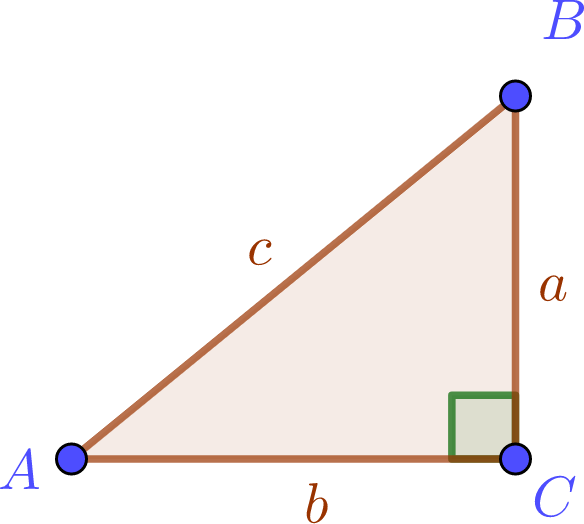
\includegraphics[width=0.3\textwidth]{pythag1}
\end{center}

There is a fundamental relation between the three lengths, which was known to the ancient Greeks. Legend has it that the relation
is due to the cult of Pythagoras, and that Pythagoras himself was so enthralled by it that he sacrificed an ox to give thanks for
its discovery --- although, as Kline points out, ``if all the legends telling of Pythagoras sacrificing an ox were true, he could
not have had time for mathematics''.\footnote{Morris Kline, \emph{Mathematics for the Nonmathematician}. Dover Publications (1985). Page 68.} In
addition, there is evidence that the theorem was known (if not proved) before the time of Pythagoras by the Babylonians, the Indians,
and the Chinese.

\begin{thm}
  If $ ABC $ is a triangle as labelled above, then $ c^2 = a^2 + b^2 $.
\end{thm}

We give two proofs, both different to the four-triangle proof which is seen in most popular books. The first is as given by Euclid in
around 300 BCE, and involves comparing areas.
\begin{center}
  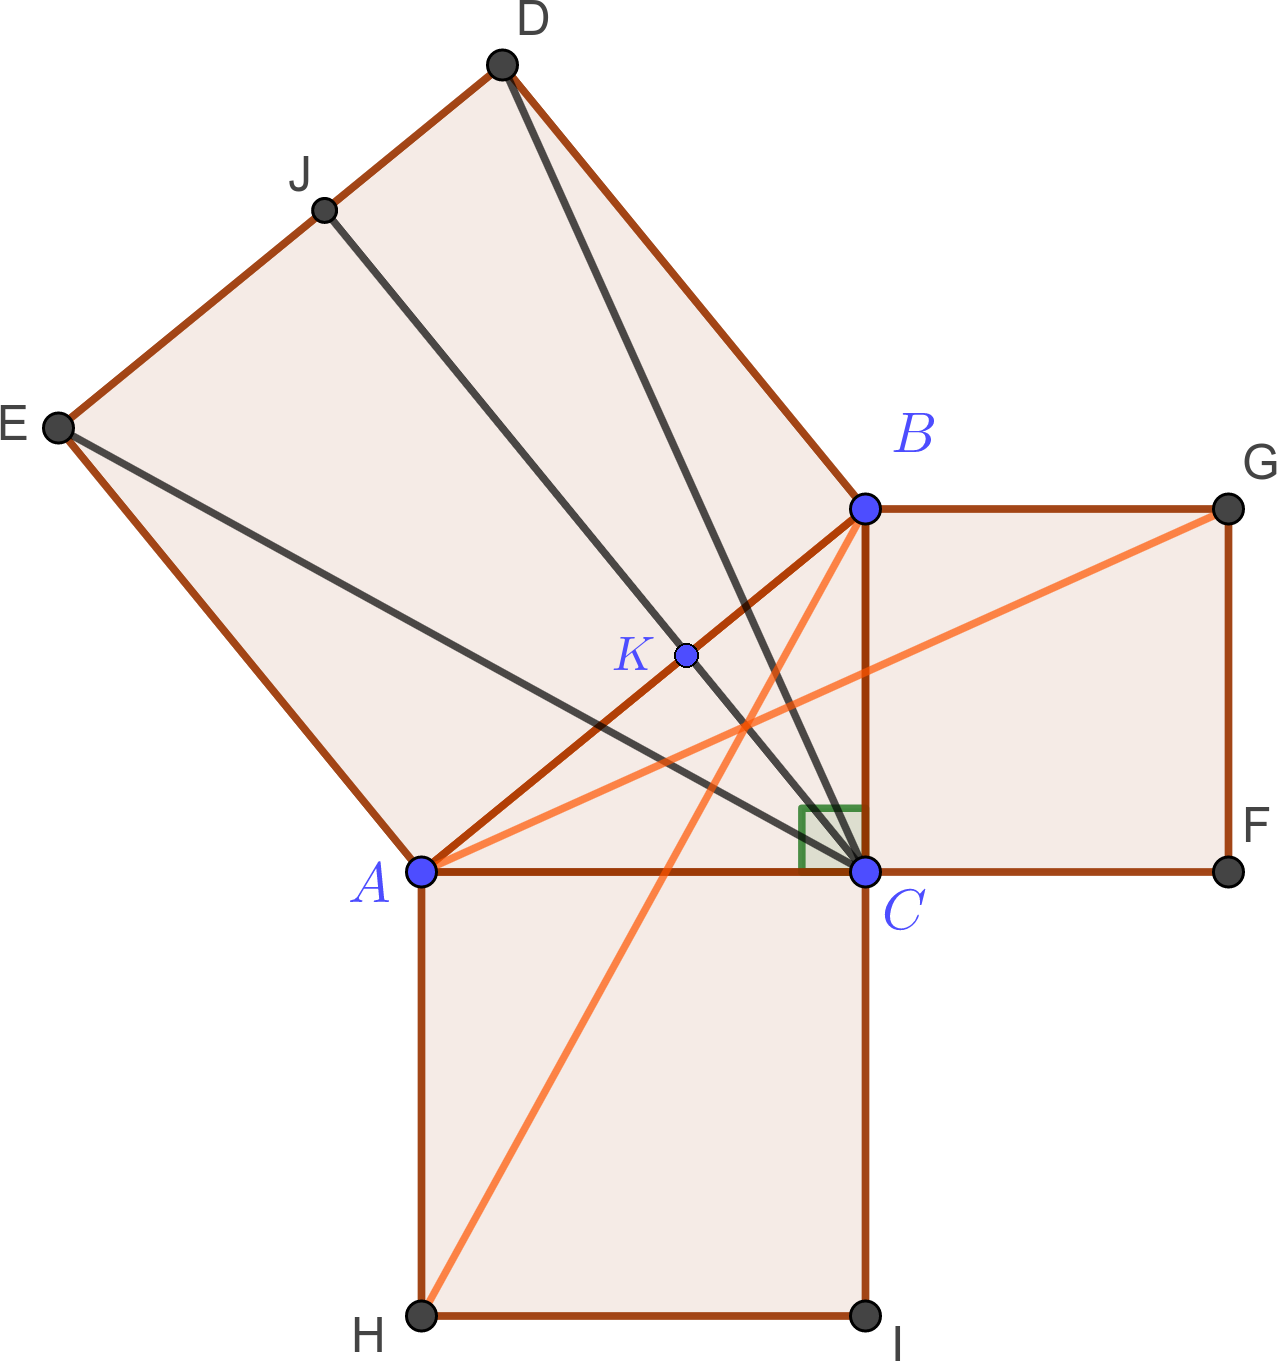
\includegraphics[width=0.4\textwidth]{pythag2}
\end{center}
\begin{proof}[Proof I (Euclid)]
  In the figure, we have:
  \begin{align*}
    \mathcal{A}(BE) &= \mathcal{A}(JB) + \mathcal{A}(JA) && \text{ (Decomposing into rectangles.)}\\
                    &= 2\mathcal{A}(BDC) + 2\mathcal{A}(AEC) && \text{ (Triangle $ DBC $ has height $ DJ $ and base $BD $, similarly for $ AEC $.)}\\
                    &= 2\mathcal{A}(BGA) + 2\mathcal{A}(BHA) && \text{ (Triangles $ BDC $ and $ BGA $ share lengths $ BG = BC $ and $ DB = AB $}\\
                    &                                        && \text{ and angles at $ B $ so are equal; similarly, $ AEC $ and $ BHA $ are equal.)}\\
                    &= \mathcal{A}(BF) + \mathcal{A}(AI) && \text{ (Triangle $ BGA $ has height $ BC $ and base $ BG $, similarly for $ BHA $.)}
  \end{align*}
\end{proof}

The second proof involves using similar triangles.
\begin{center}
  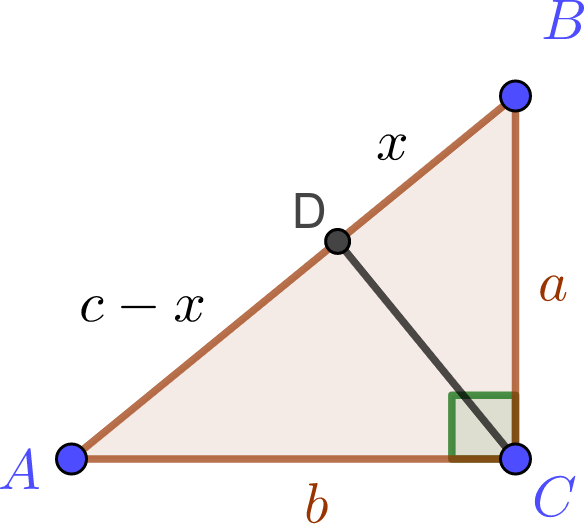
\includegraphics[width=0.3\textwidth]{pythag3}
\end{center}
\begin{proof}[Proof II]
  First, note that the three triangles $ ABC $, $ CBD $, and $ ACD $ are similar. Thus, considering $ CBD $ and $ ABD $, $ c/a = a/x $; so $ cx = a^2 $.
  Similarly, considering $ ACD $ and $ ABC $, $ c/b = b/(c - x) $; so $ c(c - x) = b^2 $. Adding the two expressions we have obtained, we
  have $ a^2 + b^2 = cx + c(c - x) = c^2 $, which is the statement of the theorem.
\end{proof}

\begin{exercise}
  This exercise asks you to prove a couple of useful theorems about triangles.
  \begin{enumerate}
    \item Show that the sum of the inscribed angles of any triangle is $ \pi $ radians. (You may use any facts
          which seem to you to be completely obvious; for example, the fact that a line crossing a pair of parallel
          lines cuts the lines at equal angles, if this fact is obvious to you.)
    \item (Inscribed angle theorem.) If $ AB $ is a chord in a circle with centre $ O $, and if $ C $ is any other
          point on the circle, then the measure of the angle $ BOA $ is twice the angle of the angle $ BCA $. (For
          example, in the following diagram $ \theta = 2\gamma $.)
          \begin{center}
            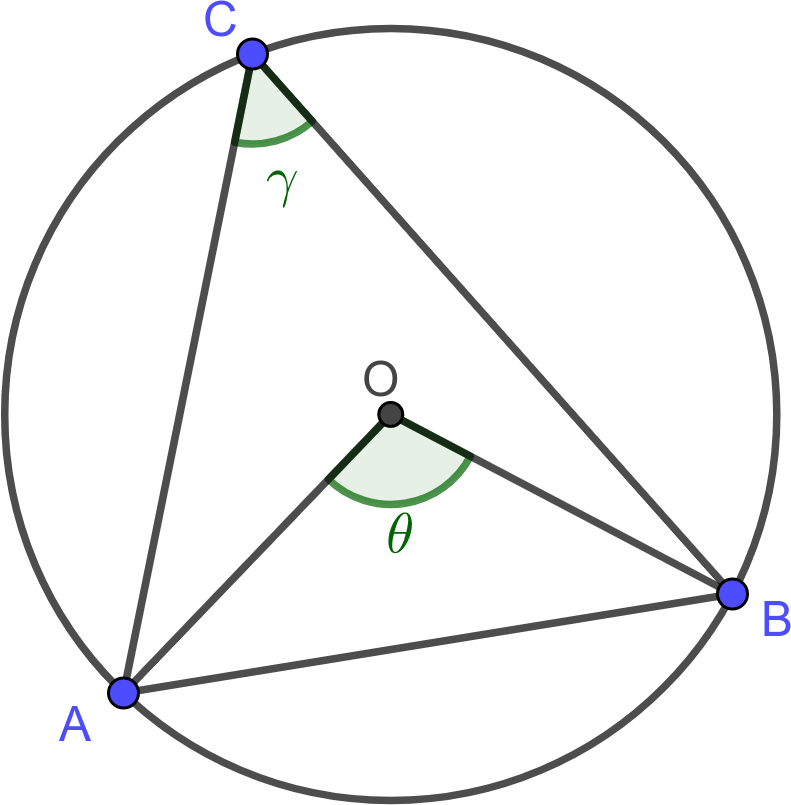
\includegraphics[width=0.3\textwidth]{inscribedanglethm}
          \end{center}
          Hint: there is an obvious line missing in the above diagram. Draw it in, and do some angle-pushing.
  \end{enumerate}
  Both of these exercises are used very often in geometry, and it is well worth committing them to memory.
\end{exercise}

\section{Definitions}
\begin{center}
  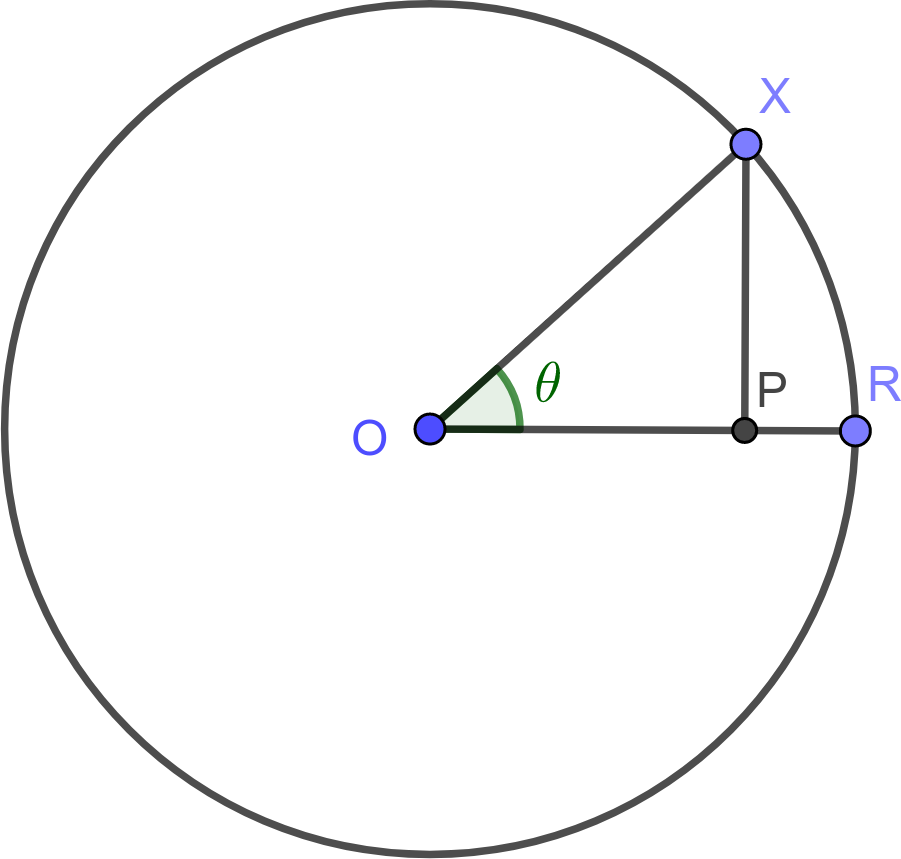
\includegraphics[width=0.3\textwidth]{fndefinitions}
\end{center}

\begin{defn}\label{defn:trig1}
  Consider a unit circle with centre $ O $ and radius $ OR $. Let $ X $ be any point on the circle, such that the angle between $ OR $ and $ OX $
  is $ \theta $ (i.e. such that the proportion of the circumference between $ R $ and $ X $ is $ \theta/2\pi $). Draw the line through $ X $,
  perpendicular to the radius $ OR $ and cutting the latter at $ P $. Then we define two functions of $ \theta $ as follows, called the \df{sine} and \df{cosine}
  functions respectively, for all $ 0 \leq \theta < \pi/2 $:-
  \begin{gather}
    \sin(\theta) = \abs{PX}\\
    \cos(\theta) = \abs{OP}.
  \end{gather}
\end{defn}

It is customary to drop the parentheses around the argument of trigonometric functions if it is a single term; for
example, $ \sin \theta $ simply means $ \sin(\theta) $. We adopt this convention whenever it is unambiguous.

It is also customary to write $ \sin^2 \theta $ in place of $ (\sin \theta)^2 $, and in general $ \sin^n \theta $
for $ (\sin \theta)^n $ whenever $ n $ is a positive integer.

Clearly, we also have $ \sin 0 = 0 $ and $ \cos 0 = 1 $.

We then extend the domains of definition of sine and cosine to the entire range $ 0 \leq \theta < 2\pi $, as follows:
\begin{equation}\label{tab:extend1}
\begin{tabular}{c|c|c|c}
  & $ \frac{\pi}{2} \leq \theta < \pi $ & $ \pi \leq \theta < \frac{3\pi}{2} $ & $ \frac{3\pi}{2} \leq \theta < 2\pi $\\\hline
  $ \sin \theta = $ & $ \sin(\pi - \theta) $ & $ -\sin(\theta - \pi)$ & $-\sin(2\pi - \theta) $\\
  $ \cos \theta = $ & $ -\cos(\pi - \theta) $ & $ - \cos (\theta - \pi) $ & $ \cos(2\pi - \theta) $.
\end{tabular}
\end{equation}

Drawing the graphs of $ y = \sin x $ (red) and $ y = \cos x $ (blue) for $ 0 \leq x < 2\pi $, we obtain the
following picture.
\begin{center}
  \fbox{\begin{tikzpicture}
    \begin{axis}[
      axis lines = center,
      ymax = 1.5, ymin = -1.5,
      xtick={1.5708, 3.14159, 4.7124, 6.28},
      xticklabels={$\frac{\pi}{2}$,$\pi$,$\frac{3\pi}{2}$,$2\pi$},
      xlabel = $ x $,
      ylabel = $ y $
    ]
      \addplot[domain = 0:2*pi, color = red] {sin(deg(x))};
      \addplot[domain = 0:2*pi, color = blue] {cos(deg(x))};
    \end{axis}
  \end{tikzpicture}}
\end{center}

Finally, we extend the domains of definition to the entire real line by declaring that for all real $ \theta $, the identities
\begin{gather}
  \sin \theta = \sin (\theta + 2n\pi)\text{ and}
  \cos \theta = \cos (\theta + 2n\pi)
\end{gather}
hold (where $ n $ is any integer). This simply implies that the graphs of the two functions repeat every $ 2\pi $; hence the graphs
as drawn above can be extended as far as we like in either direction by just making shifted copies of the bit we already drew.
\begin{center}
  \fbox{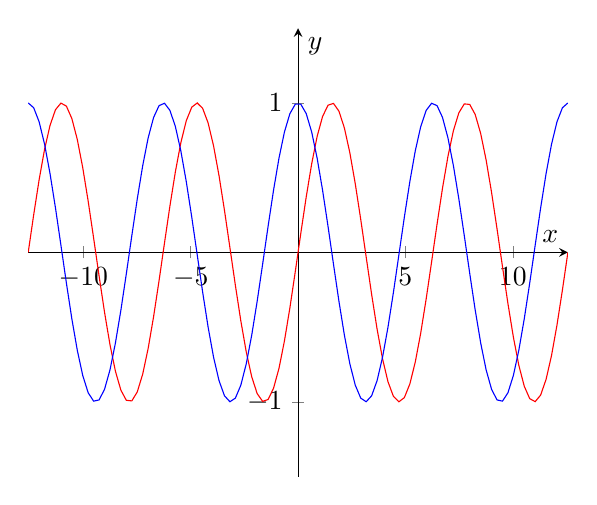
\begin{tikzpicture}
    \begin{axis}[
      axis lines = center,
      ymax = 1.5, ymin = -1.5,
      xtick={},
      xlabel = $ x $,
      ylabel = $ y $
    ]
      \addplot[domain = -4*pi:4*pi, color = red, samples=100] {sin(deg(x))};
      \addplot[domain = -4*pi:4*pi, color = blue, samples=100] {cos(deg(x))};
    \end{axis}
  \end{tikzpicture}}
\end{center}


\begin{exercise}\label{ex:geomdefn}
  Consider the unit circle again, call $ PX $ positive whenever $ X $ lies above the $ OR $ axis and negative whenever $ X $ lies below that
  axis. Then call $ OP $ positive whenever $ P $ lies on the segment $ OR $ and negative when $ P $ lies on the opposite side of $ R $. Show
  that if we define $ \sin \theta $ and $ \cos \theta $ by $ PX $ and $ OP $ respectively for all $ 0 \leq \theta < 2\pi $, keeping signs
  consistent, then the resulting functions agree with our definition above.
\end{exercise}

\begin{prp}\label{thm:basicids}
  The following identities always hold.
  \begin{enumerate}
    \item $ \sin 2n\pi = 0 $ and $ \cos 2n\pi = 1 $ for all integers $ n $.
    \item $ \sin^2 \theta + \cos^2 \theta = 1 $ for all $ \theta $.
    \item $ -1 \leq \sin \theta \leq 1 $ and $ -1 \leq \cos \theta \leq 1 $ for all $ \theta $.
    \item $ \sin (-\theta) = -\sin \theta $ and $ \cos (-\theta) = \cos \theta $ for all $ \theta $.
    \item $ \cos \theta = \sin (\theta + \pi/2) $.
    \item $ \sin (\pi - \theta) = \sin \theta $ and $ \cos(\pi - \theta) = -\cos \theta $.
  \end{enumerate}
\end{prp}
\begin{proof}\leavevmode
  \begin{enumerate}
    \item $ \sin 2n\pi = \sin(0 + 2n\pi) = \sin 0 = 0 $. A similar calculation holds for cosine.
    \item When $ 0 \leq \theta < \pi/2 $, the statement follows from an application of Pythagoras' theorem
          to the right triangle $ OPX $. When $ \pi/2 \leq \theta < \pi $,
            \begin{displaymath}
              \sin^2 \theta + \cos^2 \theta = \sin^2(\pi - \theta) + (-\cos (\pi - \theta))^2 = 1
            \end{displaymath}
            (since $ 0 \leq \pi - \theta < \pi/2 $); similar arguments show that the statement holds for all $ 0 \leq \theta < 2\pi $.
            If $ \theta $ is not in this range, then $ \theta = \theta' + 2n\pi $ for some integer $ n $ and some $ \theta' $ that
            does lie in that range; since $ \sin (\theta' + 2n\pi) = \sin \theta' $, and $ \cos (\theta' + 2n\pi) = \cos \theta' $, we
            can apply what we have already proved in this case as well.
    \item For $ 0 \leq \theta < \pi/2 $, the two functions are defined using the lengths $ PX $ and $ OP $ which
          are positive and always less than 1. For all other values of $ \theta $, the functions are defined in
          terms of the values on this interval and are not scaled beyond a negative sign; so both functions are
          bounded above by 1 and below by $ -1 $.

          Alternatively, note that by (2) above, $ \sin^2 \theta \leq 1 $ and $ \cos^2 \theta \leq 1 $ for all $ \theta $.
    \item Note that $ \sin(-\theta) = \sin(2\pi - \theta) = -\sin \theta $, and $ \cos(-\theta) = \cos(2\pi - \theta) = \cos \theta $ (by
          the final column of table \ref{tab:extend1}).
    \item Suppose $ 0 \leq \theta < \pi/2 $. Then, considering the following diagram, we perform some angle-pushing.
          \begin{center}
            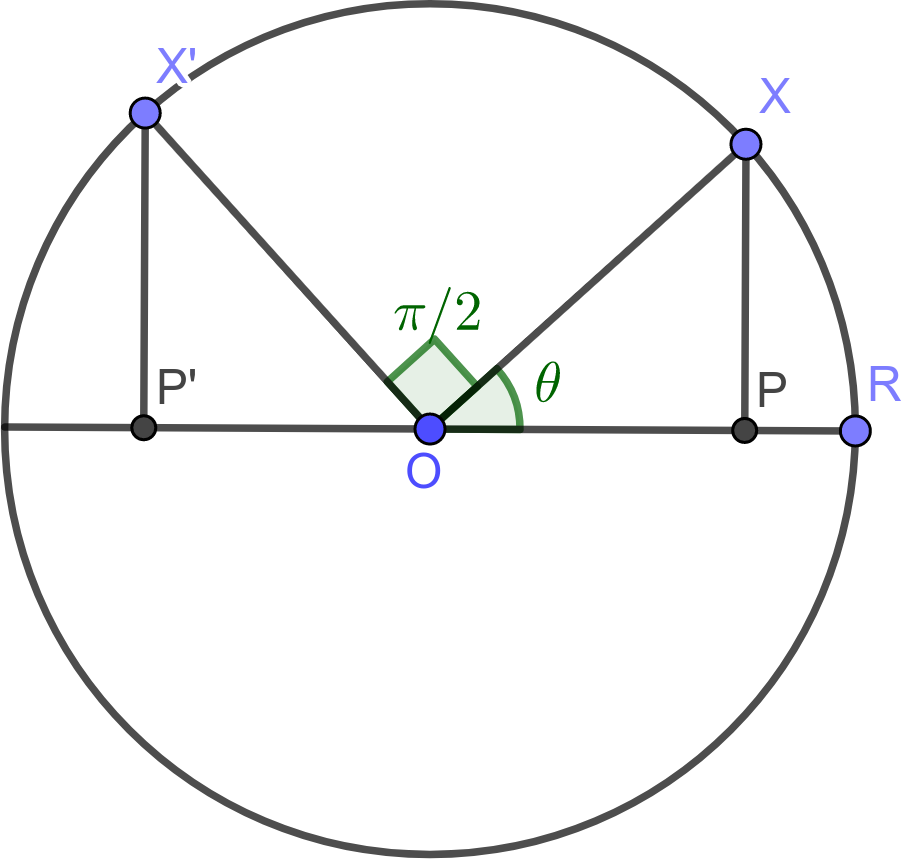
\includegraphics[width=0.3\textwidth]{shifting}
          \end{center}
          The angle $ \angle X'OP' $ has magnitude $ \frac{\pi}{2} - \theta $; hence the other angle in the right
          triangle $ X'OP' $ has magnitude $ \theta $ (since the angle-sum of triangles is $ \pi $). The two triangles
          $ XOP $ and $ X'OP' $ share all three of their angles and so are similar, and share an edge length (the radius
          of the circle) and so are equal, with lengths $ \abs{X'P'} = \abs{OP} $ and $ \abs{OP'} = \abs{XP} $. But $ \abs{X'P'} = \sin(\theta + \pi/2) $,
          and $ \abs{OP} = \cos \theta $; hence the proposition holds in this case.

          If $ \pi/2 \leq \theta < \pi $, then $ \pi \leq \theta + \pi/2 < 3\pi/2 $ and $ \sin(\theta + \pi/2) = -\sin(\theta + \pi/2 - \pi) $;
          then (applying the case we have already proved) $ -\sin(\theta - \pi/2) = -\cos(\theta - \pi) = \cos \theta $ as required. We extend
          the proof to all $ 0 \leq \theta < 2\pi $ using similar arguments, and then conclude it holds for all $ \theta $ by periodicity.
    \item Here, we apply table \ref{tab:extend1} in the reverse and simplify, if needed, using (1), (4), and periodicity.
  \end{enumerate}
\end{proof}

\begin{thm}\label{thm:ratios}
  If $ ABC $ is a right triangle such that the right angle is at $ C $, and $ \alpha $ is the interior angle at $ A $, then
    \begin{gather}
      \sin \alpha = \frac{\abs{BC}}{\abs{AB}} = \frac{\text{opposite}}{\text{hypotenuse}} \text{ and}\\
      \cos \alpha = \frac{\abs{AC}}{\abs{AB}} = \frac{\text{adjacent}}{\text{hypotenuse}}.
    \end{gather}
\end{thm}
\begin{proof}
  Construct a similar triangle $ A'B'C' $ by scaling every length of $ ABC $ by $ 1/\abs{AB} $; drawing a circle
  with radius 1 and centre $ A $, we see that $ \abs{B'C'} = \cos \alpha $ and $ \abs{A'C'} = \sin \alpha $ (taking
  the base radius to be $ A'C' $ and applying our original definition \ref{defn:trig1}). But $ \abs{B'C'} = \abs{BC}/\abs{AB} $,
  and $ \abs{A'C'} = \abs{AC}/\abs{AB} $, so we are done.
\end{proof}

Philosophically, the above identities and theorems all follow directly from the geometric definition (exercise \ref{ex:geomdefn}). This
is simply because our functional definition of sine and cosine (based on geometry for a small interval, and then the use of symmetry and periodicity to
extend it to the whole real line) was devised so that they behave in the way we expect them to based on our intuition from previous study.

Because of this, we will simply view the \emph{functions} $ \sin $ and $ \cos $ as black boxes from now on: they have the properties that we expect
the geometric sine and cosine curves to have, and so we can use the two points of view interchangably. Thus, in what follows we will freely
use both functional (i.e. depending on the fiddly details of the definition and the tables and the extensions from intervals to the real line)
and geometric arguments to justify many of the statements we will make.

Instead of pushing the definitions further, we move on to defining some more trigonometric functions. Consider the following diagram.

\begin{center}
  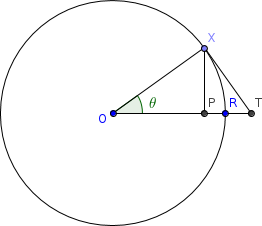
\includegraphics[width=0.3\textwidth]{tangent}
\end{center}

\begin{thm}
  If $ OXP $ is drawn in a unit circle as in the diagram, and the tangent line to the circle at $ X $ is drawn to meet the line $ OR $ at
  some point $ T $, then $ \abs{XT} = \frac{\sin \theta}{\cos \theta} $.
\end{thm}
\begin{proof}
  I claim that $ XOT $ is similar to $ POX $. This is proved by noticing that both triangles
  contain a right angle and share the angle of measure $ \theta $. Hence $ \frac{\abs{XT}}{\abs{XO}} = \frac{\abs{XP}}{\abs{OP}} $;
  but $ \abs{XO} = 1 $, $ \abs{XP} = \sin \theta $, and $ \abs{OP} = \cos \theta $, so we are done.
\end{proof}

Motivated by this theorem, we make the following
\begin{defn}
  The \df{tangent} function is the function $ \tan $ that is defined by
  \begin{displaymath}
    \tan \theta = \frac{\sin \theta}{\cos \theta}
  \end{displaymath}
  for all $ \theta \neq \frac{\pi}{2}n $ where $ n $ is an odd integer (since $ \cos \frac{\pi}{2}n $ is zero for odd $ n $).
\end{defn}

The following theorem is useful in calculus.
\begin{thm}
  For $ -\pi/2 < \theta < \pi/2 $, $ 1 < \frac{\sin x}{x} < \cos x $. In particular, as $ x \to 0 $, $ \frac{\sin x}{x} \to 1 $.
\end{thm}
\begin{center}
  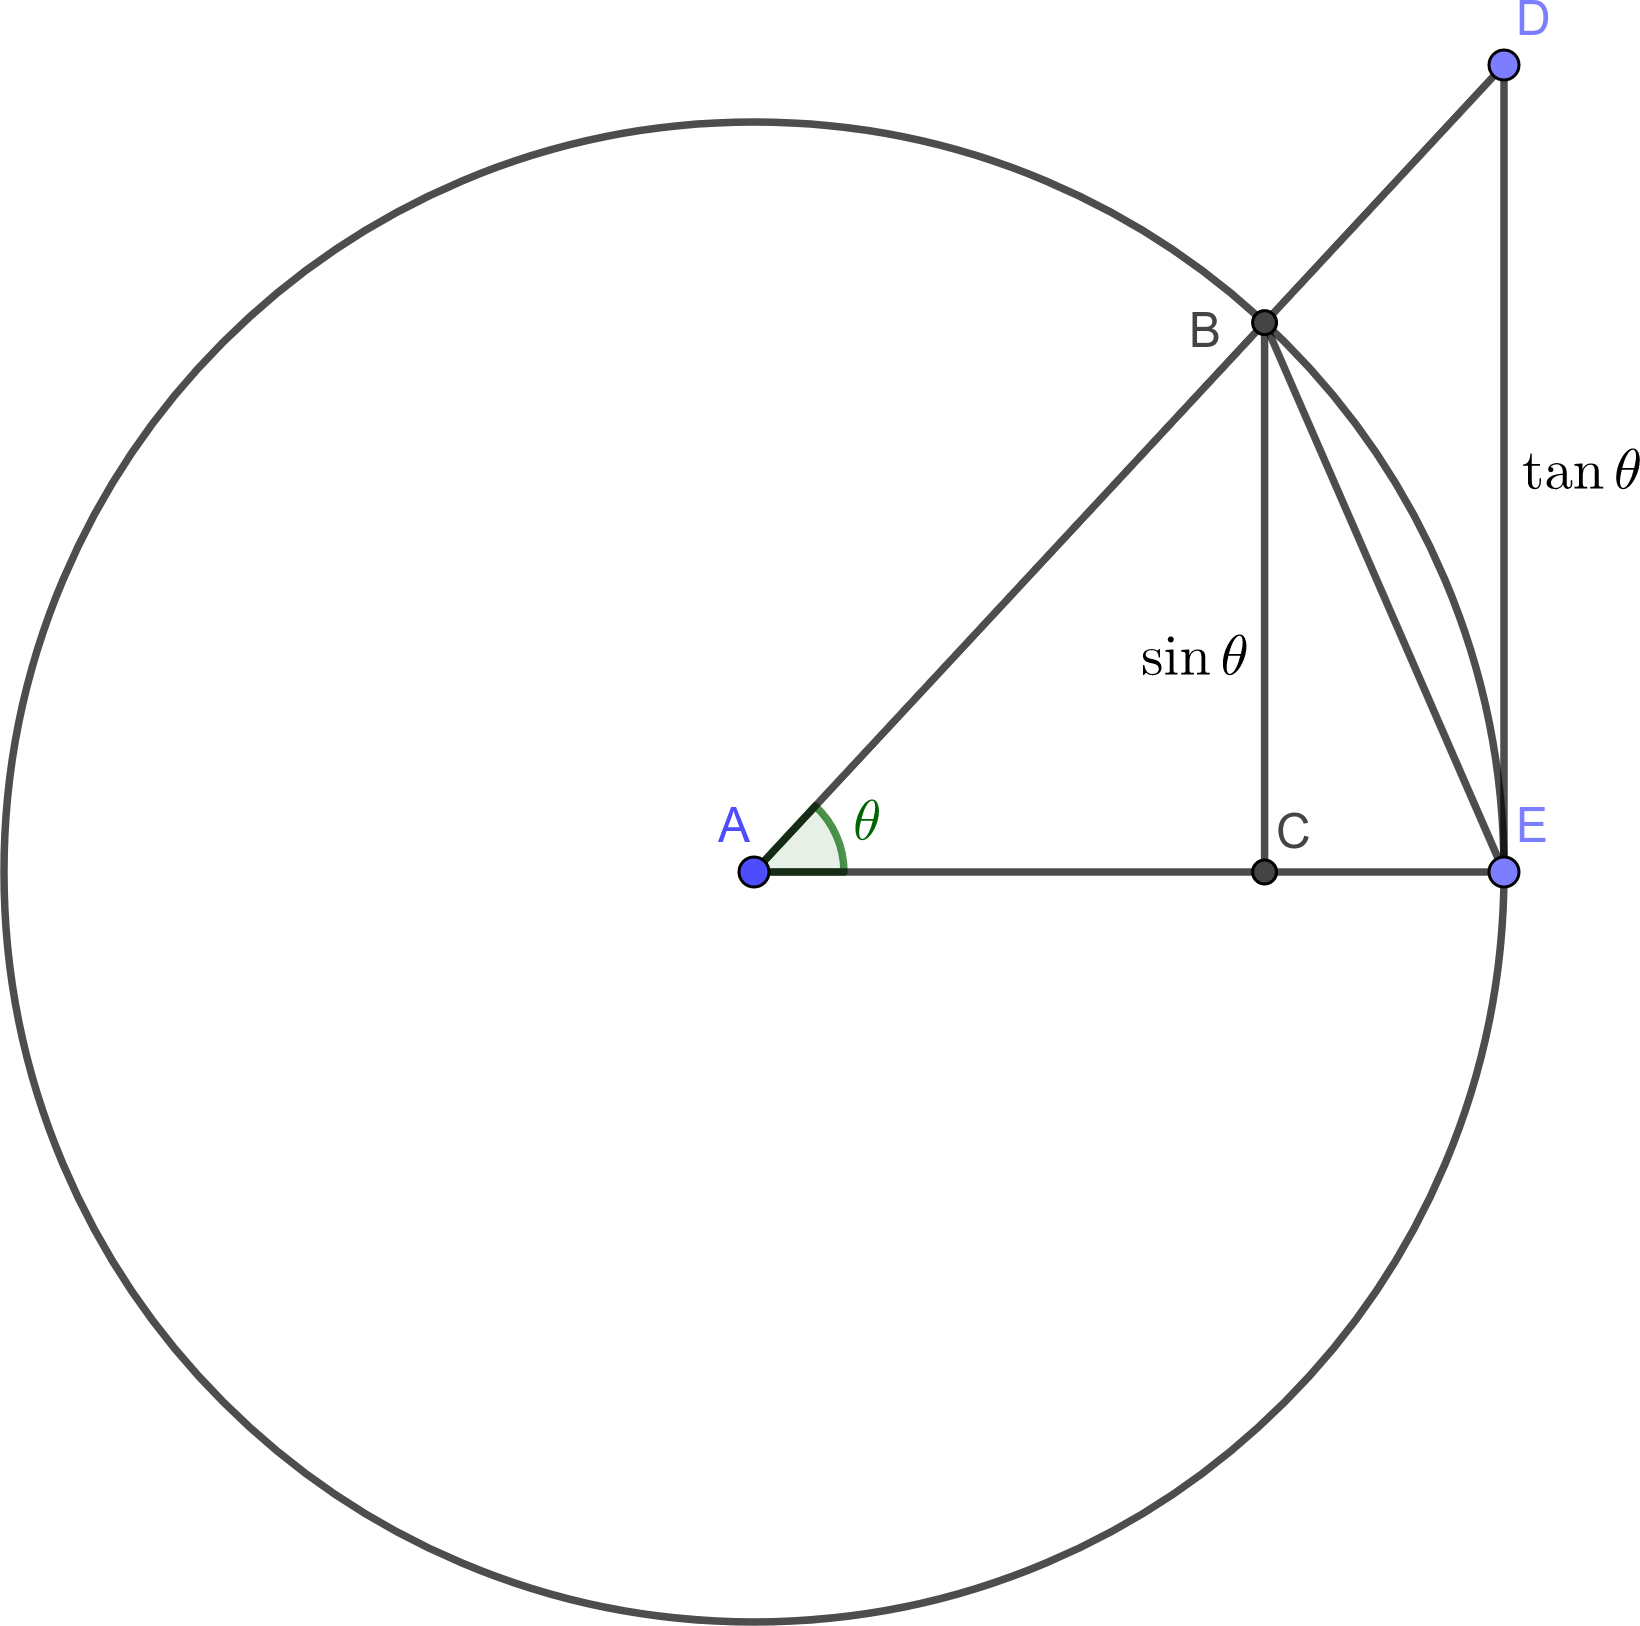
\includegraphics[width=0.3\textwidth]{sinelimit}
\end{center}
\begin{proof}
  For $ \theta > 0 $, we can use the diagram above. We have that $\mathcal{A}(\triangle ABC) = \frac{1}{2} \sin \theta $,
  that $ \mathcal{A}(\sector ABC) = \frac{\theta}{2} $, and that $ \mathcal{A}(ADE) = \frac{1}{2}\tan \theta $. By comparison
  of these areas, we have $ \frac{1}{2}\sin \theta \leq \frac{1}{2}\theta \leq \frac{1}{2}\tan \theta $ and
  hence $ 1 \leq \frac{\theta}{\sin \theta} \leq \cos \theta $.

  If $ \theta < 0 $ then $ -\theta > 0 $; we then have $ \frac{\theta}{\sin \theta} = \frac{-\theta}{\sin(-\theta)} $. Applying
  the part we have already proved, we have $ 1 \leq \frac{-\theta}{\sin(-\theta)} \leq \frac{1}{\cos(-\theta)} $. Replacing $ \cos(-\theta) $
  with $ \cos \theta $, allowed because of proposition \ref{thm:basicids}, we have the desired result for negative $ \theta $.
\end{proof}

\begin{exercise}
  Here are some revision problems from your earlier studies that should help you remember
  the mechanical aspects of applying trigonometry.
  \begin{enumerate}
    \item To measure the width $ BC $ of a straight river, a surveyor starts at $ C $ and walks
          along the bank to a point $ A $. He finds that the distance between $ A $ and $ C $
          is \SI{50}{\metre}, and the angle at $ A $ is \ang{20}. What is the width of the river?
    \item Before the advent of modern technology, it was still possible to make rough calculations
          of the circumference and radius of the earth. For example, the Alexandrian mathematician
          Eratosthenes calculated the circumference of the earth in around 200~BCE. Carry out the
          following programme to arrive at Eratosthenes' estimate.
          \begin{enumerate}
            \item First, note that the sun is far enough away for the light rays arriving at the earth to be almost
                  parallel. At the summer solstice, light hits the town of Syene so that the bottom
                  of a deep well is fully illuminated; conclude that the sun is immediately overhead.
            \item In Alexandria, \SI{800}{\kilo\metre} further north, a \SI{1}{\metre} vertical stick casts
                  a shadow of \SI{13}{\centi\metre}. Compute the angle at which the sun's rays are hitting
                  the stick.
            \item Thus compute the angle at the centre of the earth between the radii of the planet at Alexandria
                  and Syene. What is the circumference of the earth?
          \end{enumerate}
    \item Alternatively, suppose an astronomer climbs Mt Kaukau (height: \SI{445}{\metre} above sea level) and uses
          an inclinometer to measure the angle between a vertical line and her line of sight to the horizon. Suppose
          that this angle turns out to be \ang{89}. What is the radius of the earth, and hence its circumference?
  \end{enumerate}
\end{exercise}

\section{Taxonomy of Functions}
For the remainder of these notes, we only consider angles $ 0 \leq \theta < 2\pi $ unless otherwise stated. This is because
all of the interesting theory occurs in this case, and extending results to arbitrary $ \theta $ is tedious and doesn't present
any inherent complexity. The reader is invited to keep in mind our definitions from above, and to fill in on her own those
places where a negative sign or some other modification may be needed to make a result hold in general.

Consider now the following diagram based on our definitions above, where the tangent line $ XT $ to the unit circle has been
extended to meet the vertical line at $ B $; we also drop a perpendicular line from $ X $ onto the vertical line at $ A $.
Our goal is to work out how most of the new lengths we can play with depend on the trigonometric functions we have already
defined; the reader is encouraged to annotate the diagram with the names of the various functions, like $ \tan $, as they
are defined. A complete diagram is given at the end of the section.
\begin{center}
  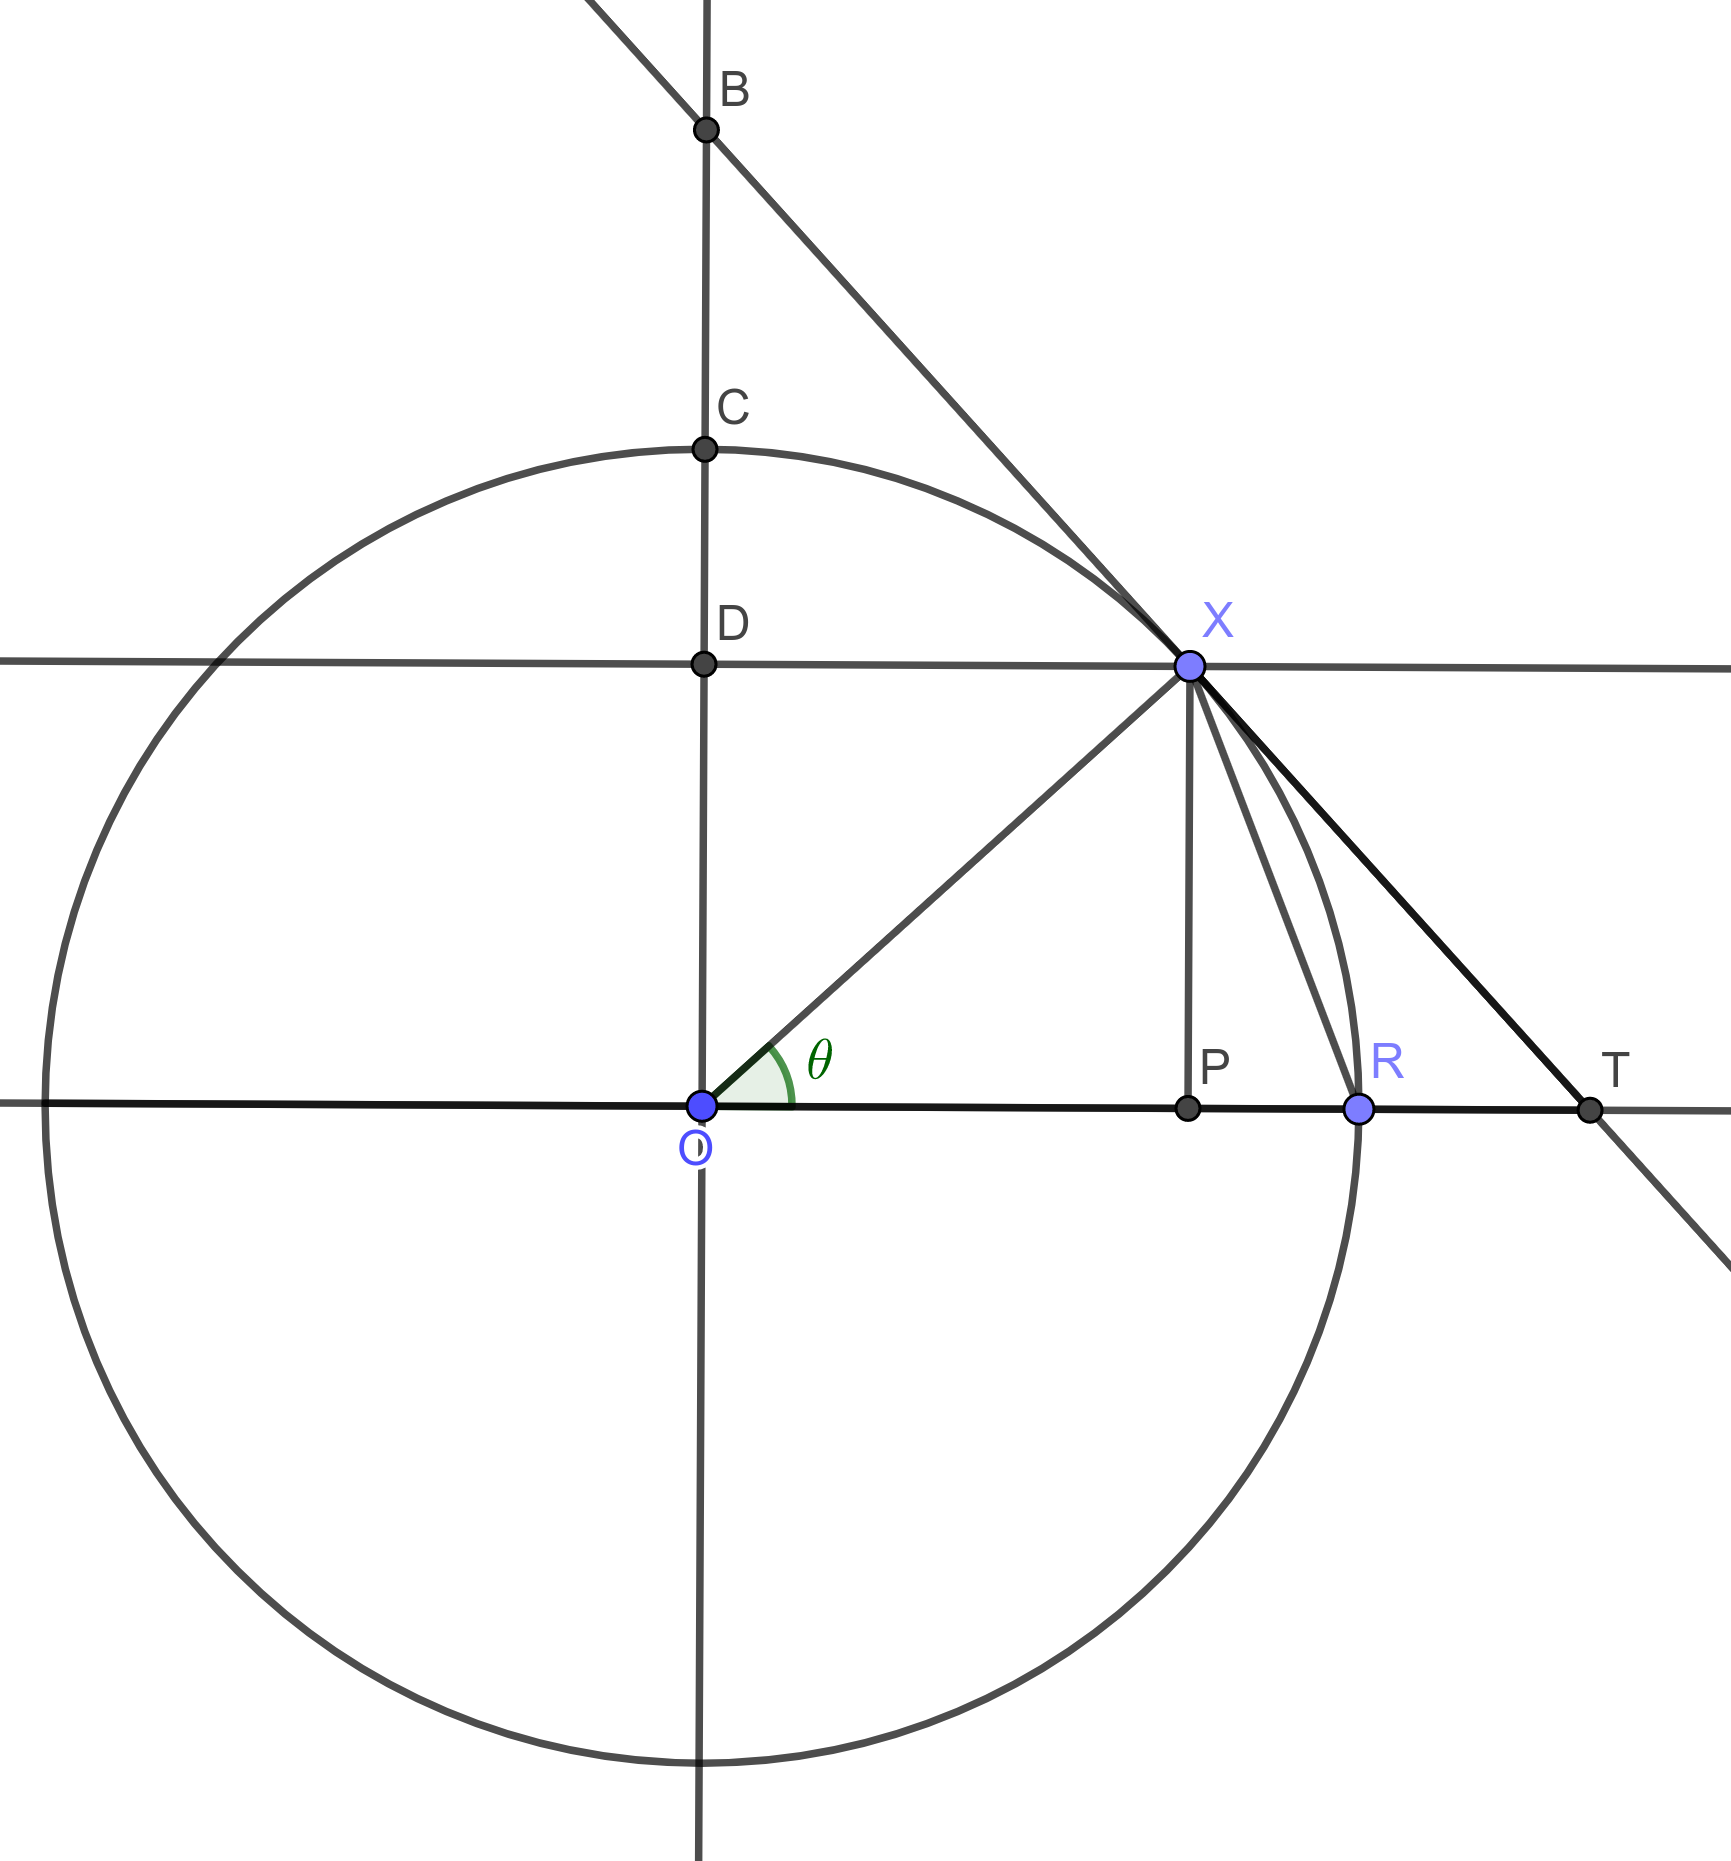
\includegraphics[width=0.5\textwidth]{taxonomy}
\end{center}

\subsection{Reciprocal Functions}
Firstly, we calculate the length of $ OT $. Consider the triangle $ OXT $; we can calculate its area in two different ways,
recalling that the area of a triangle is one half of the base times the height.
\begin{displaymath}
  \mathcal{A}(OXT) = \frac{1}{2}\abs{XT}\abs{OX} = \frac{1}{2}\abs{OT}\abs{PX}
\end{displaymath}
However, $ \abs{XT} = \tan \theta $, $ \abs{OX} = 1 $, and $ \abs{PX} = \sin \theta $. Hence we
have $ \tan \theta = \abs{OT}\sin \theta $; but $ \tan \theta = \frac{\sin \theta}{\cos \theta} $,
so $ \abs{OT} = \frac{1}{\cos \theta} $.
\begin{defn}
  The \df{secant} function is defined by $ \sec \theta = \abs{OT} = \frac{1}{\cos \theta} $.
\end{defn}

We next calculate $ \abs{BX} $. Note that $ DBX $ and $ PXT $ are similar triangles, and so $ \frac{\abs{BX}}{\abs{DX}} = \frac{\abs{XT}}{\abs{PT}} $.
Substituting in what we know, this becomes
\begin{equation}\label{eqn:cotan1}
  \frac{\abs{BX}}{\cos \theta} = \frac{\tan \theta}{\abs{PT}};
\end{equation}
but $ PXT $ is a right triangle and so, applying the Pythagorean theorem,
\begin{displaymath}
  \abs{PT} = \sqrt{\tan^2 \theta - \sin^2 \theta} = \sqrt{\frac{\sin^2 \theta}{\cos^2 \theta} - \sin^2 \theta} = \sin \theta \sqrt{\frac{1}{\cos^2 \theta} - 1},
\end{displaymath}
or (substituting into equation \ref{eqn:cotan1})
\begin{displaymath}
  \frac{\abs{BX}}{\cos \theta} = \frac{\tan\theta}{\sin\theta \sqrt{\frac{1}{\cos^2 \theta} - 1}}.
\end{displaymath}
Cancelling $ \tan \theta = \sin \theta/\cos \theta $,
\begin{displaymath}
  \abs{BX} = \frac{1}{\sqrt{\frac{1}{\cos^2 \theta} - 1}}.
\end{displaymath}
To simplify further, recall that $ \sin^2 \theta + \cos^2 \theta = 1 $, and so (dividing by $ \cos^2 \theta $)
\begin{equation}\label{eqn:tansecid}
  \tan^2 \theta + 1 = \frac{1}{\cos^2 \theta} = \sec^2 \theta.
\end{equation}
Hence $ \abs{BX} = \frac{1}{\sqrt{\tan^2 \theta}} = \frac{1}{\tan \theta} $.

\begin{defn}
  The \df{cotangent} function is defined by $ \cot \theta = \abs{BX} = \frac{1}{\tan \theta} $.
\end{defn}

Our next trick is to calculate $ \abs{OB} $. Again, we use similar triangles: $ OBT $ is similar to $ PXT $. In
particular, $ \frac{\abs{OB}}{\abs{OT}} = \frac{\abs{PX}}{\abs{PT}} $. But $ \abs{OT} = \sec \theta $, $ \abs{PX} = \sin \theta $,
and $ \abs{PT} = \sin \theta \sqrt{\sec^2 \theta - 1} = \sin \theta \tan \theta = \frac{\sin^2 \theta}{\cos \theta} $. Hence
\begin{displaymath}
  \abs{OB} = \abs{OT} \frac{\abs{PX}}{\abs{PT}} = \sec \theta \frac{\sin \theta}{\sin^2 \theta/\cos \theta} = \frac{1}{\sin \theta}.
\end{displaymath}

\begin{defn}
  The \df{cosecant} function is defined by $ \csc \theta = \abs{OB} = \frac{1}{\sin \theta} $.
\end{defn}

\begin{exercise}
  Show the pretty identity that $ \sec^2 \theta \csc^2 \theta = \sec^2 \theta \csc^2 \theta $. (Hint: apply Pythagoras to $ OBT $.)
\end{exercise}

\subsection{Historical Functions}
\begin{exercise}\leavevmode
  \begin{enumerate}
    \item By applying Pythagoras' theorem to $ BOT $, show that $ \cot^2 \theta + \tan^2 \theta + 2 = \csc^2 \theta + \sec^2 \theta $,
          and conclude by equation \ref{eqn:tansecid} that $ \cot^2 \theta + 1 = \csc^2 \theta $.
    \item By imitating the proof of equation \ref{eqn:tansecid} (i.e. using the identity $ \sin^2 \theta + \cos^2 \theta = 1 $), show
          that $ \cot^2 \theta + 1 = \csc^2 \theta $.
  \end{enumerate}
\end{exercise}

A few easy lengths follow, which only have names for historical reasons.
\begin{defn}\leavevmode
  \begin{enumerate}
    \item The \df{versine} function is defined by $ \versin \theta = \abs{PR} = 1 - \cos \theta $.
    \item The \df{coversine} function is defined by $ \cvs \theta = \abs{CD} = 1 - \sin \theta $.
    \item The \df{exsecant} function is defined by $ \exsec \theta = \abs{RT} = \sec \theta - 1 $.
    \item The \df{excosecant} function is defined by $ \excsc \theta = \abs{BC} = \csc \theta - 1$.
  \end{enumerate}
\end{defn}

\begin{exercise}
  Taking inspiration from our proofs above showing that the reciprocal trig functions correspond
  to lengths, show the following identities involving the historical trig functions.
  \begin{enumerate}
    \item $ \exsec \theta = \excsc \theta \tan \theta $
    \item $ (\versin \theta)(\cvs \theta) = \sin^2 \theta $
  \end{enumerate}
\end{exercise}

\subsection{Chords}
Finally, we compute $ \abs{XR} $. We have
\begin{displaymath}
  \abs{XR}^2 = \sin^2 \theta + \versin^2 \theta = \sin^2 \theta + (1 - \cos \theta)^2 = \sin^2 \theta + 1 - 2\cos \theta + \cos^2 \theta = 2 - 2\cos \theta.
\end{displaymath}

\begin{defn}\label{defn:chord}
  The \df{chord} function is defined by $ \crd \theta = \abs{XR} = \sqrt{2 - 2\cos \theta} $.
\end{defn}

\subsection{Summary of the Taxonomy}
\begin{center}
  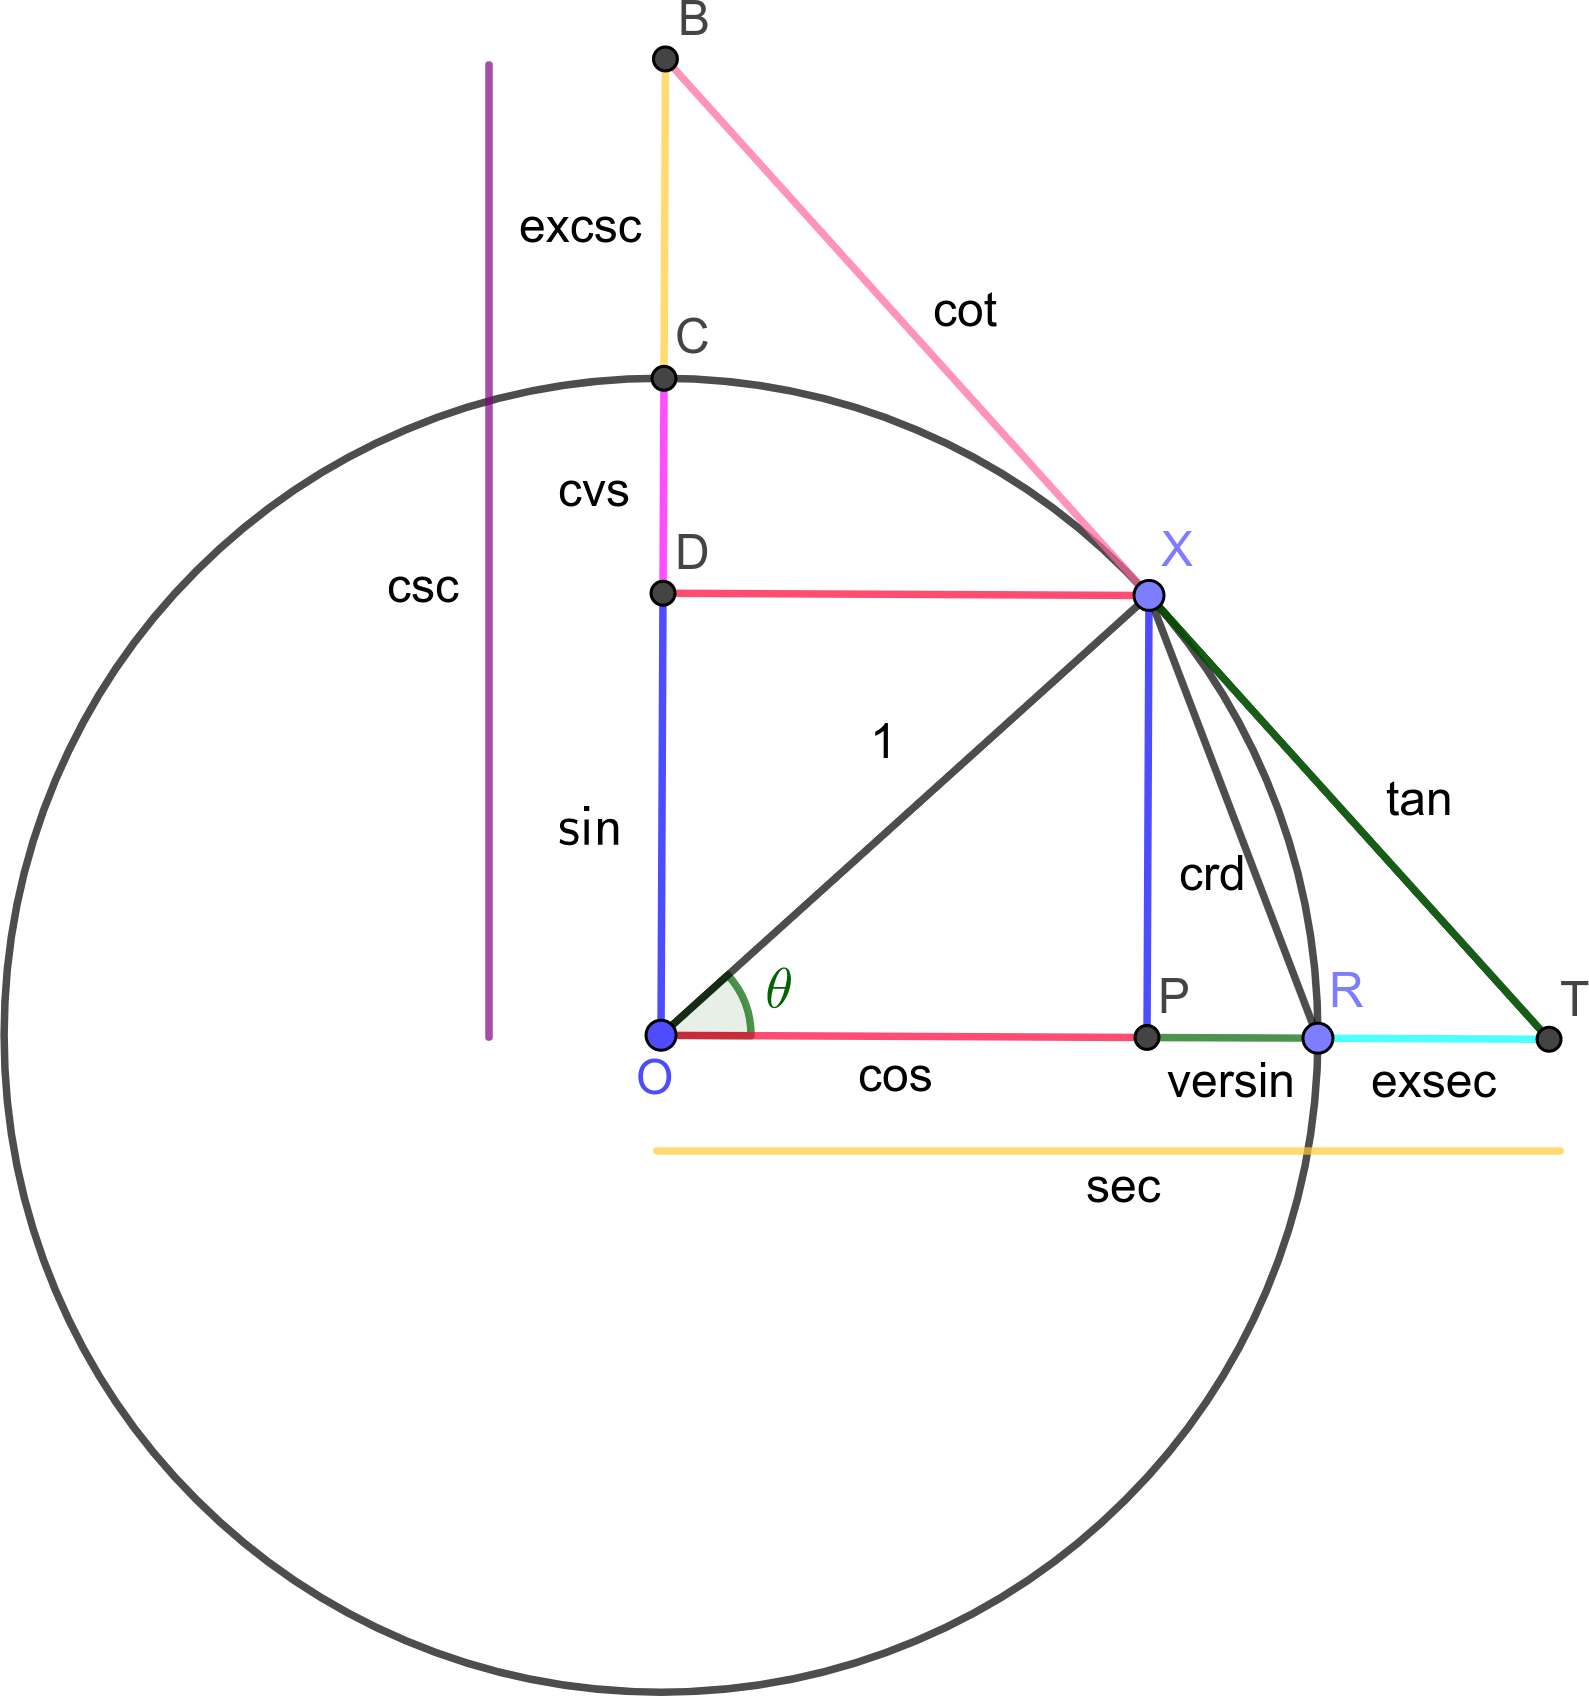
\includegraphics[width=0.5\textwidth]{taxonomyall}
\end{center}
We have the following definition, which summarises all the definitions we have made.
\begin{defn}\leavevmode
  \begin{enumerate}
    \item \textbf{Basic Functions}
      \begin{enumerate}
        \item $ \sin \theta = \abs{PX} $ (sine)
        \item $ \cos \theta = \abs{OP} $ (cosine)
        \item $ \tan \theta = \abs{XT} = \frac{\sin \theta}{\cos \theta} $ (tangent)
      \end{enumerate}
    \item \textbf{Reciprocal Functions}
      \begin{enumerate}
        \item $ \csc \theta = \abs{OB} = \frac{1}{\sin\theta} $ (cosecant)
        \item $ \sec \theta = \abs{OT} = \frac{1}{\cos\theta} $ (secant)
        \item $ \cot \theta = \abs{BX} = \frac{1}{\tan\theta} = \frac{\cos\theta}{\sin\theta} $ (cotangent)
      \end{enumerate}
    \item \textbf{Historical Functions}
      \begin{enumerate}
        \item $ \versin \theta = \abs{PR} = 1 - \cos \theta $ (versine)
        \item $ \cvs \theta = \abs{CD} = 1 - \sin \theta $ (coversine)
        \item $ \exsec \theta = \abs{RT} = \sec \theta - 1 $ (exsecant)
        \item $ \excsc \theta = \abs{BC} = \csc \theta - 1$ (excosecant)
      \end{enumerate}
    \item \textbf{Other Functions}
      \begin{enumerate}
        \item $ \crd \theta = \abs{RX} = \sqrt{2 - 2\cos \theta} $ (chord)
      \end{enumerate}
  \end{enumerate}
\end{defn}
Of these, the basic functions and the reciprocal functions are the most useful and
the only ones worth learning.

We also restate the following identities for convenience. Since the second two follow
immediately from the first, and the first is a trivial application of Pythagoras' theorem,
the reader is advised not to try to memorise them.
\begin{thm}
  For all angles $ \theta $,
  \begin{enumerate}
    \item $ \sin^2 \theta + \cos^2 \theta = 1 $,
    \item $ \tan^2 \theta + 1 = \sec^2 \theta $, and
    \item $ 1 + \cot^2 \theta = \csc^2 \theta $.
  \end{enumerate}
\end{thm}

\section{Identity Fishing}
Recall that if we consider the function $ \exp $ which maps $ x \mapsto e^x $, then we have the addition rule $ \exp(x + y) = \exp(x) \exp(y) $. Our
goal in this section is to derive similar rules for the basic trigonometric functions.

\begin{thm}\leavevmode\label{thm:sumids}
  Suppose $ \alpha $ and $ \beta $ are angles. Then:
  \begin{enumerate}
    \item $ \sin(\alpha + \beta) = \sin \alpha \cos \beta + \cos \alpha \sin \beta $
    \item $ \cos(\alpha + \beta) = \cos \alpha \cos \beta - \sin \alpha \sin \beta $
  \end{enumerate}
\end{thm}
\begin{proof}
  We prove the formulae for angles in the range $ 0 \leq \alpha < \pi/2 $ and $ 0 \leq \beta \pi/2 $, and this
  result can be generalised to all $ \theta $ using the same methods we have used before.

  For cosine, consider the following diagram.\footnote{Both this proof and the one given in the exercise below are due to Leonard M. Smiley, University of Alaska Anchorage, \url{http://math.uaa.alaska.edu/~smiley/trigproofs.html} (retrieved via Archive.org on 14 Sept 2018).}
  \begin{center}
    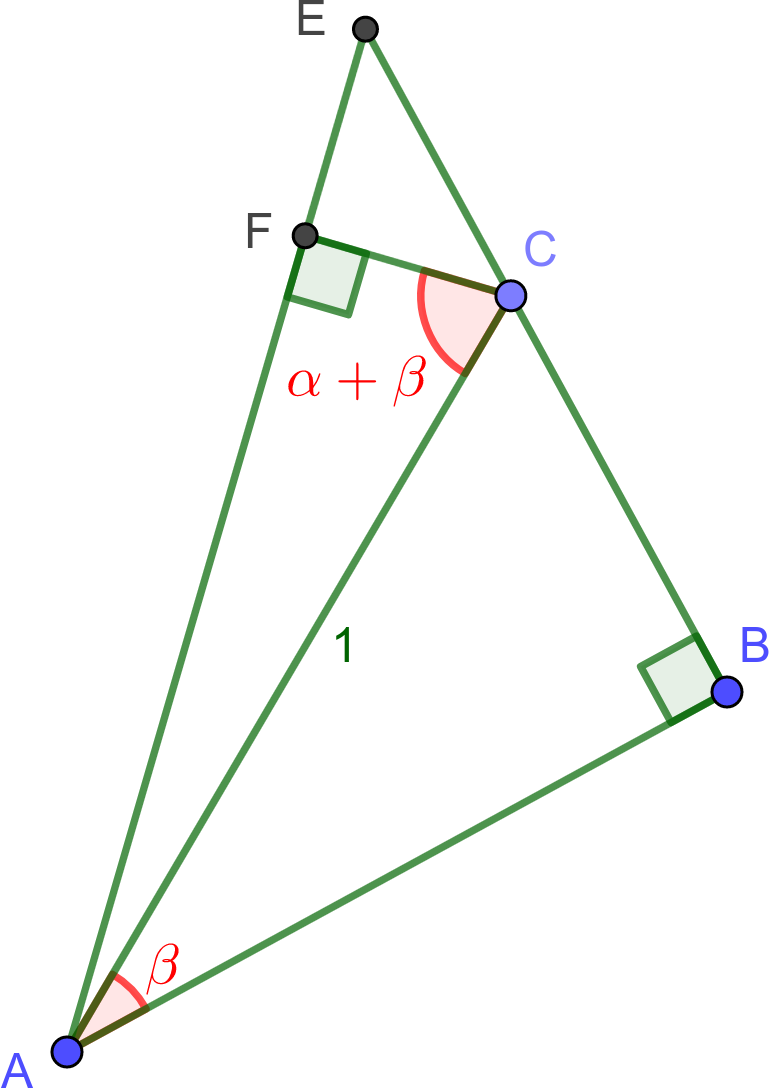
\includegraphics[width=0.3\textwidth]{cosinesum}
  \end{center}
  We have two triangles, where $ ABC $ has an angle $ \beta $ and hypotenuse $ \abs{AC} = 1 $. From $ C $ we measure an angle $ \alpha + \beta $,
  and extend this line to meet a line from $ C $ at a right angle (so both interior angles at $ F $ are right). Hence $ \abs{AB} = \cos\beta $,
  $ \abs{BC} = \sin \beta $, and $ \abs{FC} = \cos(\alpha + \beta) $. I claim that the interior angle at $ E $ is simply $ \alpha $; this
  can be seen by writing the interior angle of $ EFC $ at $ C $ as $ \pi - (\alpha + \beta) + (\pi/2 - \beta) = \pi/2 - \alpha $ and then
  using the fact that the angle sum of a triangle is $ \pi $. Using this fact and the length of $ FC $, we have that
  \begin{displaymath}
    \abs{EC} = \frac{\cos (\alpha + \beta)}{\sin \alpha}.
  \end{displaymath}
  Then by taking side ratios of the large triangle $ ABE $ we have $ \frac{\abs{AB}}{\abs{BE}} = \frac{\sin \alpha}{\cos \alpha} $, and hence
  \begin{displaymath}
    \frac{\sin \alpha}{\cos \alpha} = \frac{\cos \beta}{\frac{\cos (\alpha + \beta)}{\sin \alpha} + \sin \beta},
  \end{displaymath}
  which is rearranged to obtain $ \cos(\alpha + \beta) = \cos \alpha \cos \beta - \sin \alpha \sin \beta $ as required.
\end{proof}

\begin{exercise}
  Use the following diagram and an analagous argument to derive the sum formula for sine.
  \begin{center}
    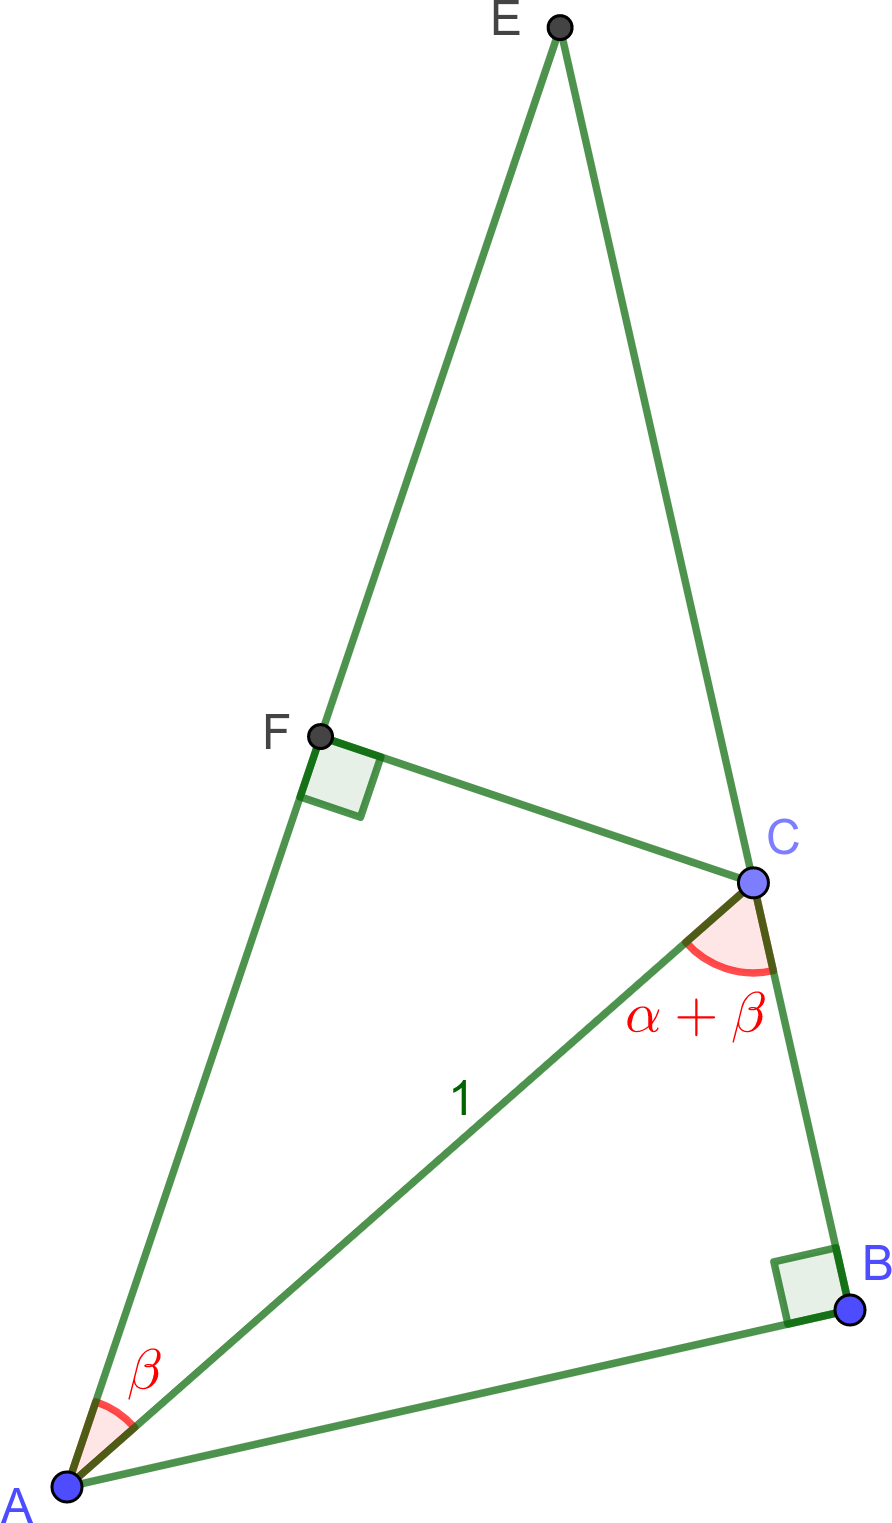
\includegraphics[width=0.3\textwidth]{sinesum}
  \end{center}
  Hint: write down $ \abs{AF} $, $ \abs{FC} $, and $ \abs{AB} $. Then show that the interior angle at $ E $ is still $ \alpha $,
  and that $ \abs{EF} = \frac{\sin\beta \cos\alpha}{\sin \alpha} $. Finally, $ \sin \alpha = \frac{\abs{AB}}{\abs{EF}} $.
\end{exercise}

\begin{cor}
  We also have the following identities:-
  \begin{enumerate}
    \item $ \sin(\alpha - \beta) = \sin \alpha \cos \beta - \cos \alpha \sin \beta $
    \item $ \cos(\alpha - \beta) = \cos \alpha \cos \beta + \sin \alpha \sin \beta $
    \item $ \tan(\alpha + \beta) = \frac{\tan \alpha + \tan \beta}{1 - \tan \alpha \tan \beta} $
    \item $ \tan(\alpha - \beta) = \frac{\tan \alpha - \tan \beta}{1 + \tan \alpha \tan \beta} $
    \item $ \sin(2\alpha) = 2 \sin \alpha \cos \alpha $
    \item $ \cos(2\alpha) = \cos^2 \alpha - \sin^2 \alpha = 1 - 2\sin^2 \alpha = 2\cos^2 \alpha - 1 $.
    \item $ \tan(2\alpha) = \frac{2\tan \alpha}{1 - \tan^2 \alpha} $.
  \end{enumerate}
\end{cor}
\begin{proof}
  For (1) and (2), simply replace $ \beta $ with $ -\beta $ in theorem \ref{thm:sumids} and apply part (4) of proposition \ref{thm:basicids}.

  For (3), write $ \tan(\alpha + \beta) = \frac{\sin(\alpha + \beta)}{\cos(\alpha + \beta)} $, apply parts (1) and (2), and simplify. Then (4)
  follows in a similar way to (1) and (2) (noting that $ \tan (-\theta) = -\tan \theta $).

  For (5) and (6), set $ \beta = \alpha $ and apply theorem \ref{thm:sumids}; (7) is done in a similar way.
\end{proof}

\begin{exercise}
  Show the following product identities hold.
  \begin{enumerate}
    \item $ 2 \sin \alpha \cos \beta = \sin(\alpha + \beta) + \sin(\alpha - \beta) $
    \item $ 2 \cos \alpha \sin \beta = \sin(\alpha + \beta) - \sin(\alpha - \beta) $
    \item $ 2 \cos \alpha \cos \beta = \cos(\alpha + \beta) + \cos(\alpha - \beta) $
    \item $ 2 \sin \alpha \sin \beta = \cos(\alpha - \beta) - \cos(\alpha + \beta) $ (note reversed $ \pm $)
  \end{enumerate}
  Find an expression for $ \tan \alpha \tan \beta $ in terms of $ \cos $.
\end{exercise}
\begin{exercise}
  Show the following half-angle identities hold.
  \begin{enumerate}
    \item $ \sin^2 \left(\frac{\alpha}{2}\right) = \frac{1 - \cos \alpha}{2} $
    \item $ \cos^2 \left(\frac{\alpha}{2}\right) = \frac{1 + \cos \alpha}{2} $
    \item $ \tan^2 \left(\frac{\alpha}{2}\right) = \frac{1 - \cos \alpha}{1 + \cos \alpha} $
  \end{enumerate}
  To remove the power of two on the left, we must take the square root of the right in each case. This root
  can have two signs: it may be positive, or negative, depending on the value of $ \alpha $. Classify all the
  relevant cases. (For which $ \alpha $ is $ \sin \alpha/2 $ positive, and for which $ \alpha $ is it negative? Repeat for all three.)
\end{exercise}
\begin{exercise}
  Show the following sum identities hold.
  \begin{enumerate}
    \item $ \sin \alpha + \sin \beta = 2\sin \frac{\alpha + \beta}{2} \cos \frac{\alpha - \beta}{2} $
    \item $ \sin \alpha - \sin \beta = 2\cos \frac{\alpha + \beta}{2} \sin \frac{\alpha - \beta}{2} $
    \item $ \cos \alpha + \cos \beta = 2\cos \frac{\alpha + \beta}{2} \cos \frac{\alpha - \beta}{2} $
    \item $ \cos \alpha - \cos \beta = -2\sin \frac{\alpha + \beta}{2} \sin \frac{\alpha - \beta}{2} $ (note negative)
  \end{enumerate}
\end{exercise}

Finally, we prove the following aesthetic identity.
\begin{thm}
  If $ x + y + z = \pi $, then $ \sin 2x + \sin 2y + \sin 2z = 4\sin x \sin y \sin z $.
\end{thm}
\begin{proof}
  First, note that since $ z = \pi - x - y $, we have $ \sin z = \sin(x + y) $ and $ \cos z = -\cos(x + y) $. This follows
  from the facts $ \sin \theta = \sin(\pi - \theta) $ and $ \cos \theta = -\cos(\pi - \theta) $ which can be easily seen
  from symmetry in the case $ 0 \leq \theta < \pi/2 $ using the unit circle (figure), and then for all other $ \theta $ by
  applying table \ref{tab:extend1} and proposition \ref{thm:basicids}. It also follows algebraically from the definition
  (see proposition \ref{thm:basicids}).
  \begin{center}
    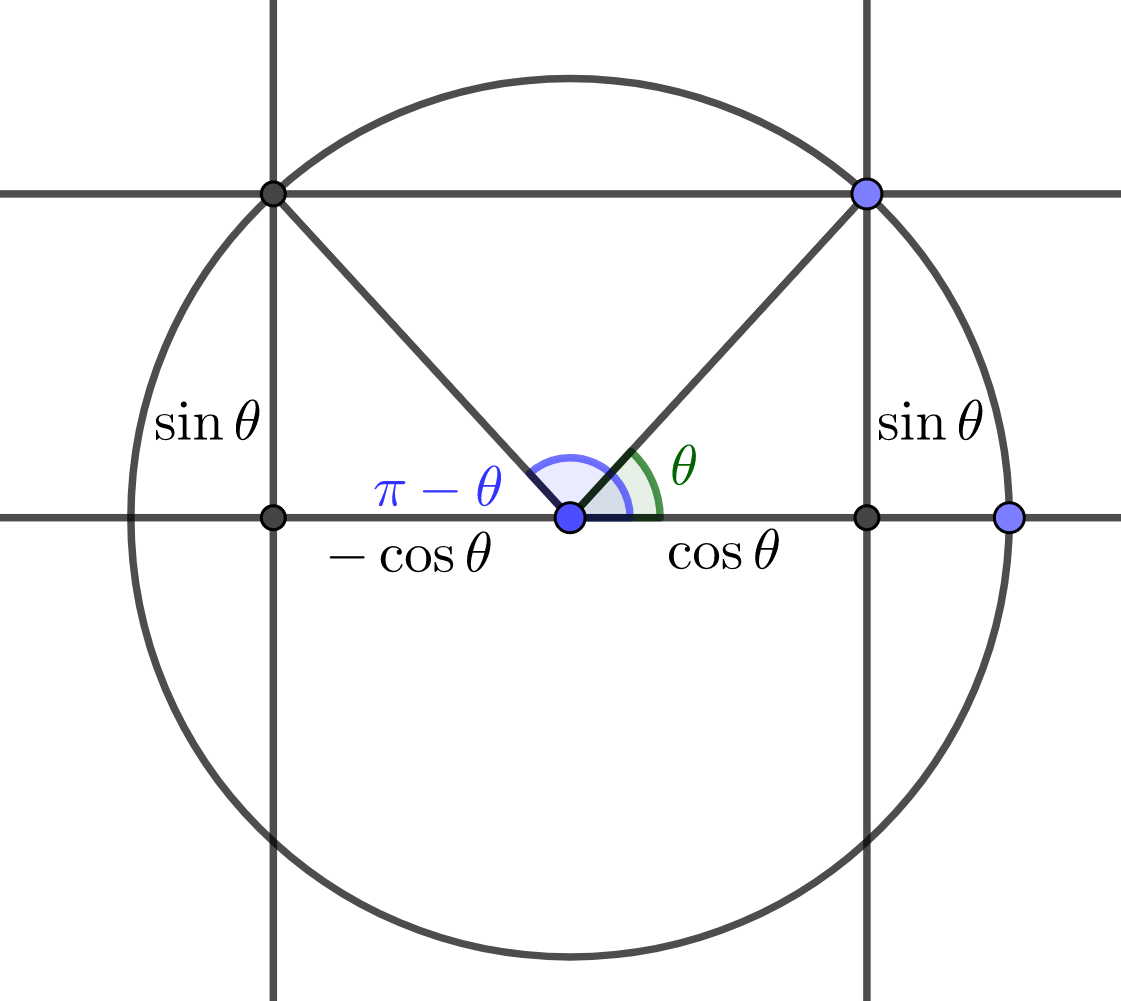
\includegraphics[width=0.3\textwidth]{piminus}
  \end{center}
  Then we argue as follows.
  \begin{align*}
    \sin 2x + \sin 2y + \sin 2x &= 2\sin(x + y)\cos(x - y) + 2\sin z \cos z\\
                                &= 2\sin z \cos(x - y) - 2\sin z \cos(x + y)\\
                                &= 2\sin z [\cos(x - y) - \cos(x + y)]\\
                                &= 2\sin z [\cos x \cos y + \sin x \sin y - \cos x \cos y + \sin x \sin y]\\
                                &= 4\sin x \sin y \sin z.
  \end{align*}
\end{proof}

\begin{exercise}
  Prove the following identities.
  \begin{enumerate}
    \item $ \sin(\alpha + \beta + \gamma) = \sin\alpha \cos\beta \cos\gamma + \cos\alpha\sin\beta\cos\gamma + \cos\alpha\cos\beta\sin\gamma - \sin\alpha\sin\beta\sin\gamma $
    \item $ \tan 3\alpha = \dfrac{3\sin\alpha - 4\sin^3 \alpha}{4\cos^3 \alpha - 3\cos\alpha} $
    \item $ \dfrac{1}{2}(\cos 2\beta - \cos 2\alpha) = \sin^2 \alpha \cos^2\beta - \cos^2\alpha \sin^2 \beta $
    \item $ \sin A + \sin B + \sin C - \sin (A + B + C) = 4\sin \frac{A + B}{2}\sin \frac{B + C}{2}\sin \frac{C + A}{2} $
    \item $ \dfrac{\sin \dfrac{B - C}{2}}{\sin \dfrac{B + C}{2}} + \dfrac{\sin \dfrac{C - A}{2}}{\sin \dfrac{C + A}{2}} + \dfrac{\sin \dfrac{A - B}{2}}{\sin \dfrac{A + B}{2}} + \dfrac{\sin \dfrac{B - C}{2}\sin \dfrac{C - A}{2}\sin \dfrac{A - B}{2}}{\sin \dfrac{B + C}{2}\sin \dfrac{C + A}{2}\sin \dfrac{A + B}{2}} = 0 $
    \item Scholarship 2018: $ \frac{\cos \theta}{1 + \sin \theta} - \frac{\sin \theta}{1 + \cos\theta} = \frac{2(\cos\theta - \sin\theta)}{1+ \sin\theta \cos \theta} $
  \end{enumerate}
\end{exercise}

\section{The Sine and Cosine Laws}
We can calculate the chord function from definition \ref{defn:chord} in a different way using the cosine rule which we learned last year.

\begin{center}
  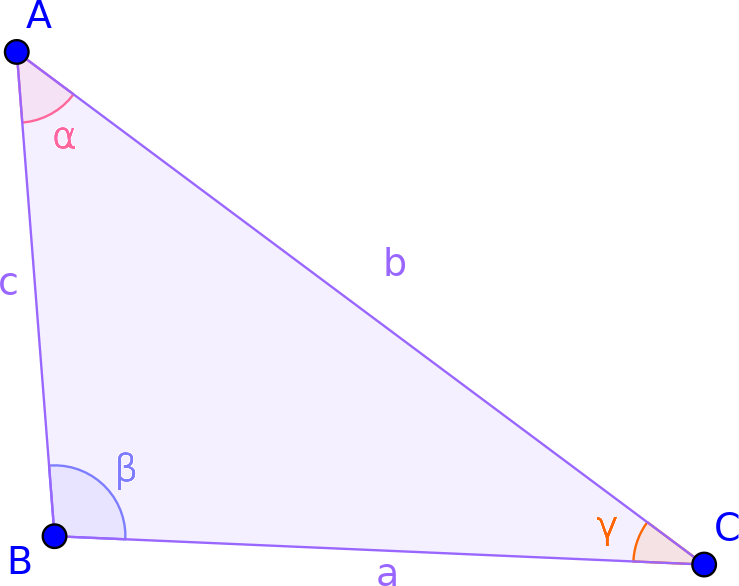
\includegraphics[width=0.2\textwidth]{trisines}
\end{center}

\begin{thm}[Law of cosines]
  If $ ABC $ is a triangle, labeled as in the picture, then $ c^2 = a^2 + b^2 - 2ab \cos \gamma $.
\end{thm}

Rather than repeat the standard proof, I will give one based on the following intersecting chord theorem.
\begin{thm}
  Suppose that $ A $, $ B $, $ C $, and $ D $ lie on a circle, and the lines $ AB $ and $ CD $ intersect at
  some point $ X $ inside the circle. Then $ \abs{AX} \abs{XB} = \abs{CX} \abs{XD} $.
\end{thm}
\begin{center}
  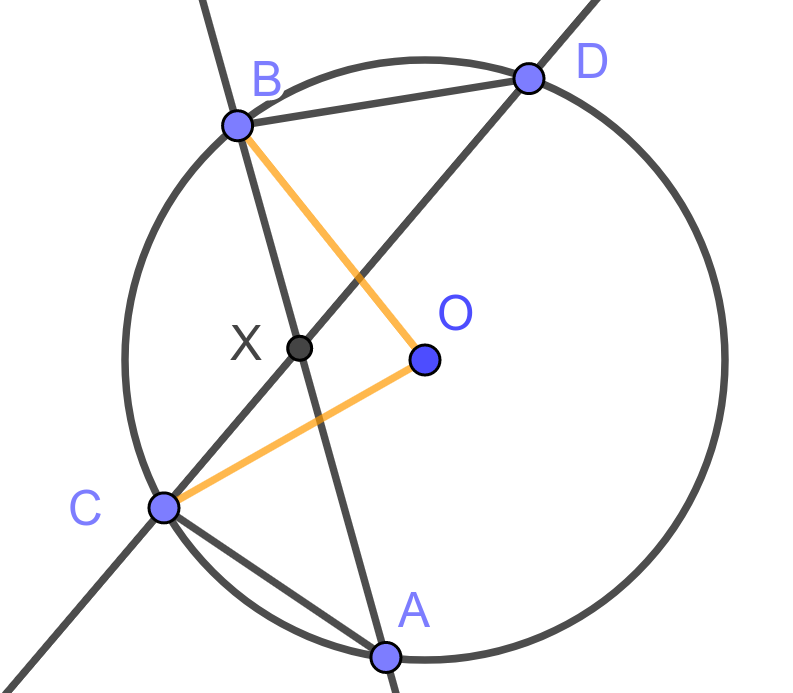
\includegraphics[width=0.3\textwidth]{ichords}
\end{center}
\begin{proof}
  I claim that $ BXD $ and $ CXA $ are similar. Clearly the two angles $ \angle DXB $ and $ \angle CXA $ are
  equal, because they are opposite. By the inscribed angle theorem, $ \angle BOC = 2\angle BDC = 2\angle BAC $
  because all three are subtended by the chord $ BC $. Hence both triangles have two equal angles, and are similar.
  The result follows from taking the side ratios $ \frac{AX}{CX} = \frac{XD}{XB} $.
\end{proof}

The law of cosines now follows immediately from the following diagram, due to Kung.\footnote{``Proof without Words: The law of cosines via Ptolemy's Theorem.'' \textit{Mathematics Magazine}, 65(2), p. 103. doi:10.1080/0025570X.1992.11995990}
\begin{center}
  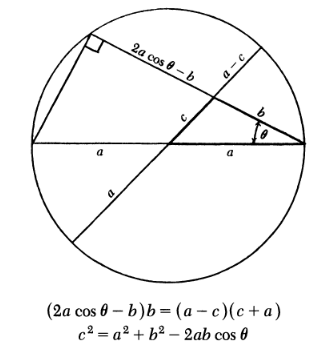
\includegraphics[width=0.4\textwidth]{cosinelawproof}
\end{center}

Then $ \crd \theta = \sqrt{1^2 + 1^2 - 2\cdot1\cdot1\cdot \cos \theta} = \sqrt{2 - 2\cos \theta} $ as before.

\begin{exercise}
  Let $ S $ be the area of the triangle $ ABC $, and let $ p $ be its half-perimeter: that is, $ p = \frac{1}{2}(a + b + c) $. Then draw
  the circle inside the triangle which is tangent to the three sides (the \df{inscribed circle}), and call its radius $ r $.
  \begin{enumerate}
    \item Show that $ S = \frac{1}{2} bc \sin \alpha $.
    \item Let $ \alpha $ be the centre of the inscribed circle. Divide the triangle into three by drawing segments
          from the three vertices to $ \alpha $. Using this, show that $ S = pr $.
    \item Show that $ \sin \alpha = \frac{2}{bc}\sqrt{p(p-a)(p-b)(p-c)} $. (Hint: this looks like the cosine rule.)
    \item Conclude that
          \begin{displaymath}
            S = \sqrt{p(p-a)(p-b)(p-c)}.
          \end{displaymath}
          (This formula is attributed to Hero of Alexandria.) Thus we have a formula for the area of a triangle which
          relies only on the lengths of the sides, and not on the height.
  \end{enumerate}
\end{exercise}

\begin{exercise}[Law of sines]
  As you will recall from last year, there is also a sine rule; we actually state here a slightly stronger
  form of it. Let $ ABC $ be a triangle labelled as in the statement for the law of cosines; draw the circle passing
  through the three vertices of the triangle (the so-called \df{circumcircle} of the triangle), and call its
  radius $ R $. Prove that
  \begin{displaymath}
    \frac{a}{\sin \alpha} = \frac{b}{\sin \beta} = \frac{c}{\sin \gamma} = 2R.
  \end{displaymath}
  Hint: try to use the inscribed angle theorem.
\end{exercise}

\section{Inverse Functions}
Suppose we draw a right triangle $ ABC $. It is clear that, if we know the three lengths, then the three angles are determined: there
is only one such triangle with the three given lengths.

In fact, since we know that one angle is a right angle, if we know the lengths of only two sides together with their position in relation
to the right angle (whether each is opposite, hypotenuse, or adjacent), then we know the length of the third side together with the angle.

This fact, which we have phrased here rather philosophically, simply means that given the ratios we found in \ref{thm:ratios},
\begin{equation}
      \sin \alpha = \frac{\abs{BC}}{\abs{AB}} = \frac{\text{opposite}}{\text{hypotenuse}} \text{ and }
      \cos \alpha = \frac{\abs{AC}}{\abs{AB}} = \frac{\text{adjacent}}{\text{hypotenuse}},
\end{equation}
there is a unique $ \alpha $ in the range $ 0 \leq \alpha < \pi/2 $ which will produce them.

More formally, we say that a function $ f(x) $ is invertible if for every possible output $ y $ in a given range, then there is precisely
one input $ x $ that will produce that output (i.e. there is a unique $ x $ such that $ y = f(x) $). If a function is invertible, then we
can define a second function $ g $ such that $ g(f(x)) = x = f(g(y)) $ for every input $ x $ and every output $ y $. We have geometrically justified, then,
that $ \sin \alpha $ and $ \cos \alpha $ are invertible on the range $ 0 \leq \alpha < \pi/2 $ --- and in fact, by the way we defined the
extensions of these functions into other intervals, they are invertible on the wider range $ -\pi/2 \leq \alpha < \pi/2 $ (in the case of $\sin$)
and $ 0 \leq \alpha < \pi $ (in the case of $\cos $).

\begin{defn}
  Suppose that we are given some real number $ x $, such that $ -1 \leq x \leq 1 $. Draw a right triangle $ ABC $ with hypotenuse $\abs{AB} = 1 $
  and side $ \abs{BC} = x $ (i.e. the right angle is at $ C $). Then we define two functions as follows:
  \begin{enumerate}
    \item The function $ \arcsin $, by writing $ \arcsin x = \alpha $ (where $ \alpha $ is the interior angle at $ A $), and
    \item The function $ \arccos $, by writing $ \arccos x = \beta $ (where $ \beta $ is the interior angle at $ B $).
  \end{enumerate}
  In other words, $ \arcsin x = \alpha $ if and only if $ -\pi/2 \leq \alpha < \pi/2 $ and $ \sin \alpha = x $, and $ \arccos x = \beta $ if
  and only if $ 0 \leq \alpha < \pi $ and $ \cos \beta = x $.

  Further, suppose we are given some real number $ y $. Define $ \arctan y = \theta $ if and only if $ -\pi/2 < \theta < \pi/2 $, and $ \tan \theta = x $.
\end{defn}

You will also see these functions written as $ \arcsin x = \sin^{-1} x $, $ \arccos x = \cos^{-1} x $, and $ \arctan x = \tan^{-1} x $; I will avoid
this notation here as it clashes with the notation $ \sin^n x = (\sin x)^n $ which we have already introduced (although philosophically speaking, if
we are to drop any notation then we should drop the latter as it is unique to trig functions, while writing a superscript $ -1 $ for inverses is very
standard across all of mathematics).

These new inverse functions are of mainly practical importance, as they allow us to reverse geometric calculations and move from lengths
to angles. We graph them here, with $ y = \arcsin x $ in red, $ y = \arccos x $ in blue, and $ y = \arctan x $ in dotted green.
\begin{center}
  \fbox{\begin{tikzpicture}
    \begin{axis}[
      axis lines = center,
      xmax = 1, xmin = -1,
      ymax = 3.1416, ymin = -1.5708,
      ytick={-1.5708, 0, 1.5708, 3.1416},
      yticklabels={$-\frac{\pi}{2} $, $0$, $\frac{\pi}{2}$, $\pi$},
      xlabel = $ x $,
      ylabel = $ y $
    ]
      \addplot[samples=100,domain = -1:1, color = red] {asin(x)/180*pi};
      \addplot[samples=100,domain = -1:1, color = blue] {acos(x)/180*pi};
      \addplot[samples=100,style=dashed,domain = -1:1, color = OliveGreen] {atan(x)/180*pi};
    \end{axis}
  \end{tikzpicture}}
\end{center}

By definition, $ \sin(\arcsin x) = \arcsin(\sin x) = 1 $ (and analagous statements hold for $ \cos $ and $ \tan $). However, the
definitions do not say anything about combinations like $ \sin(\arccos x) $ or $ \arctan(\sin x) $. It turns out that expressions
like these show up in calculus reasonably often, so we will look at them carefully.

Note that the first class of this kind of expression, those of the form $ \text{inverse}(\text{trig}(x)) $, can be turned into
`normal' equations: if $ y = \arctan(\sin x) $, then $ \tan y = \sin x $ and we can solve for $ y $ by studying the nature of
solutions of trigonometric equations. We will do this in the next section.

For now, then, we will consider only expressions consisting of an inverse function inside a normal trigonometric function.
\begin{thm}
  In general, the following identities hold:
  \begin{enumerate}
    \item $ \sin(\arccos x) = \sqrt{1 - x^2} $
    \item $ \sin(\arctan x) = \frac{x}{\sqrt{x^2 + 1}} $
    \item $ \cos(\arcsin x) = \sqrt{1 - x^2} $
    \item $ \cos(\arctan x) = \frac{1}{x^2 + 1} $
    \item $ \tan(\arcsin x) = \frac{x}{\sqrt{1 - x^2}} $
    \item $ \tan(\arccos x) = \frac{\sqrt{1 - x^2}}{x} $
  \end{enumerate}
\end{thm}
\begin{proof}
  We prove (1) and (6) here, leaving the remainder as an exercise. Consider the triangle given below.
  \begin{center}
    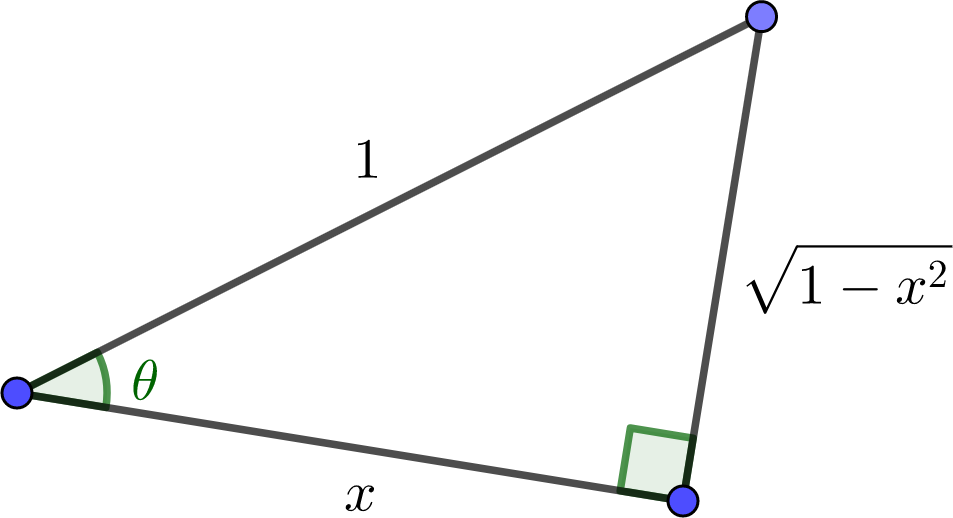
\includegraphics[width=0.3\textwidth]{invid1}
  \end{center}
  Then $ \theta = \arccos x $ (since $ \cos \theta = \frac{x}{1} $). Calculating $ \sin \theta $ and $ \tan \theta $
  we arrive at the required identities.
\end{proof}

\begin{exercise}\leavevmode
  \begin{enumerate}
    \item Prove that the identity $ \arctan x = 2\arctan(\csc \arctan x - \tan \arccot x) $ holds.
    \item Show that, if $ \arccos x + \arccos y + \arccos z = \pi $, then $ x^2 + y^2 + z^2 + 2xyz = 1 $.
  \end{enumerate}
\end{exercise}

\section{Trigonometric Equations}
The trigonometric functions are not very well-behaved with respect to the rational numbers --- they tend to map
simple inputs to complicated real numbers. However, there are a few special values which we can compute, corresponding
to triangles with simple sides.
\begin{exercise}\leavevmode\label{ex:specialtriangles}
  \begin{enumerate}
    \item \textbf{Standard special triangles.} Show, by drawing appropriate triangles, the following identities. This is not year twelve any more,
                                               so in particular you must prove that if you construct a triangle with given angles then it has the
                                               correct lengths (or vice versa, if you pick a triangle with given lengths then it has the given angles).
      \begin{enumerate}
        \item $ \sin \pi/4 = \cos \pi/4 = 1/\sqrt{2} $ and $ \tan \pi/4 = 1 $ (45-45-90)
        \item $ \sin \pi/6 = 1/2 $, $ \cos \pi/6 = \sqrt{3}/2 $, and $ \tan \pi/6 = 1/\sqrt{3} $ (60-30-90)
        \item $ \sin \pi/3 = \sqrt{3}/2 $, $ \cos \pi/3 = 1/2 $, and $ \tan \pi/6 = \sqrt{3} $ (60-30-90)
      \end{enumerate}
    \item \textbf{Magical exotic triangles.}
      \begin{enumerate}
        \item Draw an isoceles triangle with angles $ \pi/5 $, $ 2\pi/5 $, and $ 2\pi/5 $ (36-72-72), and shortest length 1.\footnote{This
              triangle is known as the \df{golden triangle}.} By bisecting one of the angles with measure $ 2\pi/5 $ and working with ratios
              of lengths of similar triangles, show that the two longer lengths $ \phi $ satisfy the equation $ 1 + \phi = \phi^2 $. (The
              measure $ \phi $ is known as the golden ratio.) Conclude that:
              \begin{enumerate}
                \item $ \sin \pi/5 = \frac{\sqrt{\phi^2 - 1/4}}{\phi} $, $ \cos \pi/10 = \frac{1}{2\phi} $, and $ \tan \pi/10 = 2\sqrt{\phi^2 - 1/4} $.
                \item $ \sin \pi/10 = \frac{1}{2\phi} $, $ \cos \pi/10 = \frac{\sqrt{\phi^2 - 1/4}}{\phi} $, and $ \tan \pi/10 = \frac{1}{2\sqrt{\phi^2 - 1/4}} $.
              \end{enumerate}
      \end{enumerate}
  \end{enumerate}
  Remark: To remember (1a) and (1b) above, cut an equilateral triangle in half.
\end{exercise}

We can also easily compute the zeroes of the trigonometric functions.
\begin{thm}\leavevmode
  \begin{enumerate}
    \item $ \sin \theta = 0 $ precisely when $ \theta = n \pi $ for arbitrary integers $ n $.
    \item $ \cos \theta = 0 $ precisely when $ \theta = n \frac{\pi}{2} $ for odd integers $ n $.
    \item $ \tan \theta = 0 $ precisely when $ \theta = n\pi $ for arbitrary integers $ n $.
  \end{enumerate}
\end{thm}
\begin{proof}
  We give the proof for $ \cos $ carefully, leaving the proof for $ \sin $ to the reader. (Note that the result for $ \tan $ follows
  directly from the result for $ \sin $.)

  From the unit circle definitions, we see that the line segment that defines $ \cos \theta $ is zero precisely when $ \theta = \pi/2 $
  or $ \theta = 3\pi/2 $. We then have, by periodicity, that $ \cos (2\pi m + \pi/2) = 0 $ and $ \cos(2\pi m + 3\pi/2) $ are all of the
  zeroes of $ \cos $ for arbitrary integers $ m $. But $ 2\pi n + \pi/2 = (4m + 1) \pi/2 $, and $ 2\pi m + 3\pi/2 = (4m + 3) \pi/2 $; and every odd number $ n $ is
  either of the form $ n = 4m + 1 $ or $ n = 4m + 3 $. The result follows.
\end{proof}

Before we can start solving trigonometric equations, we also need to take account of the periodicity of the functions. For
example, note that $ \sin \pi/4 = \sin 3\pi/4 $.

\begin{thm}\leavevmode
  In all of the following, $n $ is an arbitrary integer.
  \begin{enumerate}
    \item Suppose that $ \sin x = \sin y $. Then every $ y = n\pi + (-1)^n x $ is a solution, and every solution for $ y $ is of this form.
    \item Suppose that $ \cos x = \cos y $. Then every $ y = 2n\pi \pm x $ is a solution, and every solution for $ y $ is of this form.
    \item Suppose that $ \tan x = \tan y $. Then every $ y = n\pi + x $ is a solution, and every solution for $ y $ is of this form.
  \end{enumerate}
\end{thm}
When looking for particular solutions, it is often useful to sketch the graphs of the relevant functions; this gives far better intuition
than simply applying the formulae given here and hoping.
\begin{proof}
  We prove (1) and leave the other two as exercises. We need to check two things: (a) that $ \sin x = \sin (n\pi + (-1)^n x) $ for any integer $ n $,
  and (b) that if $ \sin x = \sin y $ then $ y $ is of the form given.

  For (a), we have two cases: either $ n = 2k $, or $ n = 2k + 1 $ for some integer $ k $ (i.e. $ n $ is either even or odd). If $ n $ is
  even, then $ \sin(n\pi + (-1)^n x) = \sin(2k\pi + (-1)^{2k} x) = \sin x $; if $ n $ is odd,
  then $ \sin(n\pi + (-1)^n x) = \sin((2k + 1)\pi + (-1)^{2k + 1}x) = \sin(2k\pi + \pi - x) = \sin(\pi - x) = \sin x $.

  For (b), note from our definitions and proposition \ref{thm:basicids} that $ \sin x = \sin y $ precisely when $ y = (\pi - \theta) + 2k\pi $
  or $ y = \theta + 2k\pi $. In the first case, $ y = (2k + 1)\pi - (-1)^{2k + 1} \theta $ and we let $ n = 2k + 1 $, and in the second case
  we let $ n = 2k $.
\end{proof}

We will now solve some trigonometric equations.
\begin{ex}
  Consider $ \sin x = \cos x $. Then $ \tan x = 1 $, and thus (by exercise \ref{ex:specialtriangles} and the above theorem) $ x = \pi/4 + n\pi $
  for arbitrary integers $ n $.
\end{ex}

\begin{ex}
  A more difficult example: consider the equation $ \sin 2x \sec 4x + \cos 2x = \cos 6x $.
  \begin{align*}
    \sin 2x \sec 4x + \cos 2x - \cos 6x &= 0\\
    \sin 2x \sec 4x + 2\sin 4x \sin 2x &= 0 && \text{ (By identity for $ \cos \alpha - \cos \beta $.)}\\
    \sin 2x (\sec 4x + 2\sin 4x) &= 0 && \text{ (So one possibility is $ \sin 2x = 0 $.)}\\
    \sec 4x + 2\sin 4x &= 0 && \text{ (Assume not, and divide through to find more solutions.)}\\
    1 + 2\sin 4x \cos 4x &= 0 && \text{ (Multiply through by $ \cos 4x $.)}\\
    1 + \sin 8x &= 0 && \text{ (Double angle formula.)}
  \end{align*}
  Hence we have two possibilities: $ \sin 2x = 0 $, and $ \sin 8x = -1 $. In the first case, one solution is $ 2x = 0 $
  and so by the theorem above all the solutions are given by $ 2x = n\pi $ (where $ n $ is an arbitrary integer); in the
  second case, one solution is $ 8x = 3\pi/2 $, and so all of them are $ 8x = n\pi + (-1)^n 3\pi/2 $ (again, $ n $ is arbitrary).

  Thus the solutions of the original equation are $ x = n\pi/2 $ and $ x = n\pi/8 + (-1)^n 3\pi/16 $ for all integers $ n $.
\end{ex}

\begin{exercise}
  Solve the following equations for $ \theta $:
  \begin{enumerate}
    \item $ \sin 2\theta = \cos \theta $
    \item $ \sin \theta + 2\cos \theta = 1 $
    \item $ \sec 4\theta - \sec 2\theta = 2 $
    \item $ \tan(\pi/4 + \phi) = 3\tan(\pi/4 - \phi) $
    \item $ \cos 5\theta + 5\cos 3\theta + 10\cos \theta = \frac{1}{2} $
    \item $ \tan 3\theta - \tan 2\theta - \tan \theta = 0 $
  \end{enumerate}
\end{exercise}

\section{Periodic Models}
The trigonometric functions are very useful for modelling periodic phenomena.
\begin{ex}
  Suppose we have a coil of wire rotating in a uniform magnetic field, like in the figure below. The induced current will oscillate
  from some maximum value $ I_\text{max} $, down to zero, and then reverse until it reaches $ -I_\text{max} $. This device, which tranforms
  mechanical (kinetic) energy into an oscillating voltage, is an AC generator and larger versions are used in most power stations
  worldwide (the only major power source which does not use such a generator is solar power).

  \begin{center}
    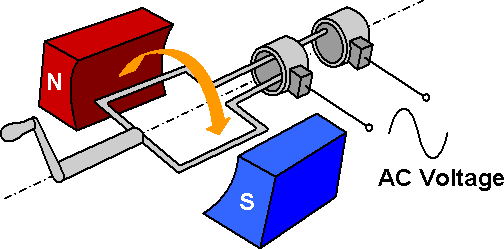
\includegraphics[width=0.5\textwidth]{acgenerator}
  \end{center}

  Since the current is generated by circular rotation, one might guess that trigonometric functions would be a good choice for
  a mathematical model of an alternating current; this guess turns out to be correct.
\end{ex}

The most general sine curve is given by
\begin{equation}
  f(t) = A\sin(\omega t - \phi) + y_0.
\end{equation}

The various constants are as follows:
\begin{itemize}
  \item The \df{amplitude}, $ A $, is the difference between the maximum and minimum values of $ f $.
  \item The \df{$ y$-shift}, $ y_0 $, is the average of the maximum and minimum values of $ f $.
  \item The \df{angular frequency}, $ \omega $, is $ 2\pi/T $ where $ T $ is the period of $ f $.
  \item The \df{phase shift}, $ \phi $, is the time at which the cycle begins.
\end{itemize}

\begin{center}
  \fbox{\begin{tikzpicture}
    \begin{axis}[
      axis lines = center,
      ymax = 1.5, ymin = -1.5,
      xmin = -0.5,
      xtick={0, 6.4},
      xticklabels={$\phi$, $\phi + 2\pi/\omega$},
      ytick={-1,0,1},
      yticklabels={$y_0 - A $, $ y_0$, $ y_0 + A $},
      xlabel = $ t $,
      ylabel = $ f(t) $,
      after end axis/.code={
        \path (axis cs:0,0)
            node [anchor=north west,yshift=-0.075cm] {$\phi$}
            node [anchor=south east,xshift=-0.075cm] {$y_0$};
    }
    ]
      \addplot[domain = -0.5:6.4, color = red] {sin(deg(x))};
    \end{axis}
  \end{tikzpicture}}
\end{center}

If we replace $ \sin $ with any trig function, we get a similar picture; further, if we replace $ \sin $
with an arbitrary function $ f $, then these parameters behave in precisely the same way: if we write
\begin{equation}
  y = Af(\omega t - \phi) + y_0.
\end{equation}
then $ A $ behaves as a stretch in the $ y$-direction, $ \omega $ acts as a stretch in the $ x$-direction,
and $ \phi $ and $ y_0 $ give $ x$- and $ y$-shifts respectively. Thus there is not much to say about
the modelling potential of trig functions in general, except to note that they behave particularly nicely
with respect to these parameters due to being bounded (in the case of $ \sin $ and $ \cos $) and periodic
(in the case of all trig functions).

\section{Epilogue: Hyperbolic Trigonometric Functions}
\begin{center}
  This section requires some knowledge of complex algebra and conic sections.
\end{center}
We will now consider a hyperbola in place of the circle we have already studied.
\begin{defn}
  The functions \df{hyperbolic sine} and \df{hyperbolic cosine} are respectively defined by
  \begin{gather*}
    \sinh u = \frac{e^u - e^{-u}}{2}\\
    \cosh u = \frac{e^u + e^{-u}}{2}.
  \end{gather*}
\end{defn}

\begin{exercise}\leavevmode
  \begin{enumerate}
    \item With reference to the polar form of complex numbers: show that $ \cos u = \frac{e^{iu} + e^{-iu}}{2} $ and
          that $ \sin u = \frac{e^{iu} - e^{-iu}}{2i} $.
    \item Hence show that $ \sinh u = -i \sin iu $ and $ \cosh u = \cos iu $.
    \item Conclude that $ \sinh $ and $ \cosh $ have imaginary periods of $ 2i\pi $.
  \end{enumerate}
\end{exercise}

\begin{exercise}\label{ex:hyperidentities}
  Define $ \tanh $, $ \sech $, $ \csch $, and $ \coth $ analagously to the circular functions. Then show that
  \begin{enumerate}
    \item $ \cosh^2 u - \sinh^2 u = 1 $,
    \item $ \sech^2 u + \tanh^2 u = 1 $, and
    \item $ \coth^2 u - \csch^2 u = 1 $.
  \end{enumerate}
\end{exercise}

\begin{exercise}
  Postulate and prove formulae for $ \cosh(u \pm v) $ and $ \sinh(u \pm v) $.
\end{exercise}

Let us now draw the hyperbola $ x^2 - y^2 = 1 $.
\begin{center}
  \fbox{\begin{tikzpicture}
    \begin{axis}[
      axis lines = center,
%       ymax = 1.5, ymin = -1.5,
      xmax = 5, xmin = -5,
      xlabel = $ x $,
      ylabel = $ y $
    ]
      \addplot[domain = 1:5, color = red, samples = 50] {sqrt(abs(x)^2 - 1)};
      \addplot[domain = 1:5, color = red, samples= 50] {-sqrt(abs(x)^2 - 1)};
      \addplot[domain = -5:-1, color = red, samples = 50] {sqrt(abs(x)^2 - 1)};
      \addplot[domain = -5:-1, color = red, samples= 50] {-sqrt(abs(x)^2 - 1)};
    \end{axis}
  \end{tikzpicture}}
\end{center}

By exercise \ref{ex:hyperidentities} above, if we let $ x = \cosh u $ and $ y = \sinh u $ then these
values satisfy the hyperbola equation. In fact, we can obtain every value on the hyperbola in this way;
for example, if $ y = \sinh u = (e^u - e^{-u})/2 $ then $ 0 = e^{2u} - 2ye^u - 1 $ and this quadratic
has nonnegative discriminant for all $ y $.

\begin{exercise}\leavevmode
  \begin{enumerate}
    \item Show that the equation above has solutions in $ u $ for all $ y $ --- in particular, that the
          roots of the quadratic are always positive (if some root $ e^u $ was nonpositive then there would
          be no such $ u $).
    \item Show that $ x = \cosh u $ has solutions for all $ x $ such that $ \abs{x} \geq 1 $.
  \end{enumerate}
\end{exercise}

Hence the hyperbolic trigonometric functions play the same role for the hyperbola as the usual functions
play for the circle.

One might now ask why it is the case that the circular functions and hyperbolic functions seem to be
related by `passing through $ \mathbb{C} $'. The answer is actually quite simple, but requires some study
of the geometry of the complex exponential function which is far beyond what we need for these notes.\footnote{See, for example, A.I. Markushevich, \emph{Theory of Functions of a Real Variable}. Revised English Edition (trans. by Richard A. Silverman). Chelsea Publishing Company (1977). Vol. 1, pages 146 to 159 (\S40-2).  }

\section*{Further Reading}
See references in text, as well as:
\begin{itemize}
  \item Marcel Berger, \emph{Geometry I} (trans. by M. Cole and S. Levy). Springer-Verlag (1994).\footnote{Particularly chapter 10.}
  \item H.S.M. Coxeter, \emph{Introduction to Geometry}. John Wiley \& Sons (1961).
  \item Paul Foerster, \emph{Trigonometry: functions and applications}. Second Edition. Addison-Wesley Publishing Co. (1977).
  \item E.W. Hobson, \emph{A Treatise on Plane Trigonometry}. Second Edition. Cambridge University Press (1897).
  \item Serge Lang and Gene Murrow, \emph{Geometry: A high-school course} Springer-Verlag (1983).
  \item Marko Petkov\v sek, Herbert S. Wilf, and Doron Zeilberger, \emph{$A = B$}. A K Peters, Ltd. (1996).
\end{itemize}

\end{document}
